\documentclass {beamer}

    \usepackage [utf8,francais,multichap] {courspda}

    \hypersetup
    {
	pdfauthor={Pierre David},
        pdfsubject={Systèmes d'exploitation},
	pdftitle={Systèmes d'exploitation},
	pdfkeywords={Systèmes d'exploitation, POSIX, fichiers, répertoires, processus, temps, signaux, tubes}
    }

    2015 -- 2016 (printemps)

    \title {Systèmes d'exploitation}

\begin {document}

%%%%%%%%%%%%%%%%%%%%%%%%%%%%%%%%%%%%%%%%%%%%%%%%%%%%%%%%%%%%%%%%%%%%%%%%%%%%%%
% PLAN
%%%%%%%%%%%%%%%%%%%%%%%%%%%%%%%%%%%%%%%%%%%%%%%%%%%%%%%%%%%%%%%%%%%%%%%%%%%%%%

\def\inc{inc1-intro}

\def\cpudb{Stanford CPU database -- \url {http://cpudb.stanford.edu/}}

\titreA {Introduction aux systèmes concurrents}

%%%%%%%%%%%%%%%%%%%%%%%%%%%%%%%%%%%%%%%%%%%%%%%%%%%%%%%%%%%%%%%%%%%%%%%%%%%%%%
% Introduction
%%%%%%%%%%%%%%%%%%%%%%%%%%%%%%%%%%%%%%%%%%%%%%%%%%%%%%%%%%%%%%%%%%%%%%%%%%%%%%

\titreB {Introduction}

\begin {frame} {Introduction}

    Qu'est-ce qu'un système concurrent~?

    \begin {quote}
	Système dans lequel plusieurs activités s'exécutent
	simultanément tout en ayant des interactions les unes avec
	les autres

    \end {quote}

    \vspace* {3mm}

    Exemples~:

    \begin {itemize}
	\item serveur (Web, base de données, jeu, etc.) répondant à
	    des requêtes de plusieurs clients «~simultanés~»
	\item système de contrôle d'un véhicule effectuant des actions
	    (débit d'essence) en fonction d'informations provenant de
	    capteurs (tachymètre)
	\item application de commerce en ligne affichant l'état du
	    stock en fonction des commandes en cours

    \end {itemize}

\end {frame}

\begin {frame} {Introduction}

    Système concurrent \implique plusieurs activités logicielles
    partagent une ou plusieurs ressources matérielles

    \vspace* {3mm}

    Deux approches~:

    \begin {enumerate}
	\item Sérialiser les traitements
	    \begin {itemize}
		\item Sérialiser en bloc \implique pas de
		    concurrence
		\item Découper les traitements et sérialiser chaque élément \\
		    Exemple~: module \texttt {asyncio} avec Python

	    \end {itemize}
	    \implique performances médiocres pour des systèmes complexes

	\item Utiliser le parallélisme sous-jacent
	    \begin {itemize}
		\item parallélisme matériel
		\item parallélisme offert par le système d'exploitation
	    \end {itemize}
	    \implique meilleure utilisation du matériel
    \end {enumerate}

    Dans la suite, on s'intéressera à la deuxième approche

\end {frame}

%%%%%%%%%%%%%%%%%%%%%%%%%%%%%%%%%%%%%%%%%%%%%%%%%%%%%%%%%%%%%%%%%%%%%%%%%%%%%%
% Motivations
%%%%%%%%%%%%%%%%%%%%%%%%%%%%%%%%%%%%%%%%%%%%%%%%%%%%%%%%%%%%%%%%%%%%%%%%%%%%%%

\titreB {Motivations}

\begin {frame} {Motivations}
    Pourquoi des systèmes concurrents (ou parallèles)~?

    \begin {enumerate}
	\item besoin de performances
	\item besoin de \emph {scalabilité}
	\item besoin de fiabilité
	\item besoin de clarté
    \end {enumerate}
\end {frame}

\begin {frame} {Motivations -- Performances}
    Amélioration des performances~:
    \begin {itemize}
	\item pour diminuer le temps de calcul

	    \vspace* {1mm}

	    Ex~: prévision météo à 3 jours en moins de 3 jours
	    de calcul...

	\item pour traiter des problèmes plus grands

	    \vspace* {1mm}

	    Ex~: prévision météo plus précise signifie~:
	    \begin {itemize}
		\item maillage plus fin
		\item plus de paramètres influant sur le calcul
	    \end {itemize}
	    \implique temps de calcul plus important

    \end {itemize}

\end {frame}

\begin {frame} {Motivations -- Performances}

    Pour aller plus vite, il faut :

    \begin {enumerate}
	\item améliorer le débit \implique récupérer les temps morts
	\item améliorer le temps de réponse \implique partager la charge
	\item améliorer le temps d'exécution \implique collaborer
    \end {enumerate}
\end {frame}

\begin {frame} {Motivations -- Performances}
    Récupérer les temps morts~:

    \begin {center}
	\includegraphics [width=.9\textwidth] {\inc/motiv-inact}
    \end {center}

    Récupération des temps morts \implique plusieurs processus

    \vspace* {3mm}

    \implique parallélisme entre  plusieurs processus dans un système
    d'exploitation
\end {frame}

\begin {frame} {Motivations -- Performances}
    Partager la charge~:

    \begin {center}
	\includegraphics [width=.9\textwidth] {\inc/motiv-part}
    \end {center}

\end {frame}

\begin {frame} {Motivations -- Performances}
    Collaborer~:

    \begin {center}
	\includegraphics [width=.9\textwidth] {\inc/motiv-collab}
    \end {center}

\end {frame}

\begin {frame} {Motivations -- Performances}
    En pratique, accroître les performances passe par~:
    \begin {itemize}
	\item le découplage des unités de traitement
	\item le découplage de la mémoire
	\item le découplage des entrées/sorties
    \end {itemize}

    \vspace* {3mm}
    \implique multi-ordinateurs
\end {frame}

\begin {frame} {Motivations -- Performances}

    Faut-il passer par le parallélisme~? \\
    L'augmentation des performances du silicium ne suffit-elle pas~?

    \vspace* {3mm}

    Augmentation des fréquences d'horloge des processeurs~:

    \begin {itemize}
	\item réduction de la durée du cycle d'horloge
	\item unités fonctionnelles du processeur plus
	    rapides
    \end {itemize}
    \implique davantage d'instructions exécutées par seconde
\end {frame}

\begin {frame} {Motivations -- Performances}
    Augmentation des fréquences d'horloge des processeurs~:

    \begin {center}
	\includegraphics [width=.9\textwidth] {\inc/cpu-freq}

	\centerline {\tiny Données : \cpudb}
    \end {center}

\end {frame}

\begin {frame} {Motivations -- Performances}
    L'augmentation de la fréquence d'horloge entraîne~:
    \begin {itemize}
	\item interférences, notamment sur des «~longues~» distances \\
	    \implique i.e. dès qu'il faut sortir du carré de silicium
	\item consommation électrique
	\item dissipation thermique
    \end {itemize}
    \vspace* {3mm}
    \implique palier\footnote {Augmentation depuis le milieu des années
    1980 : processeurs RISC} depuis le milieu des années 2000

\end {frame}

\begin {frame} {Motivations -- Performances}
    Aller au delà de l'augmentation des fréquences \implique 2 pistes

    \vspace* {3mm}

    \begin {enumerate}
	\item réduire les distances \implique augmenter la finesse de gravure
	    \begin {itemize}
		\item réduire les interférences
		\item diminuer la tension (réduire les pertes électriques)
	    \end {itemize}
	\item augmenter le nombre de transistors \implique utiliser plus
	    de place et/ou réduire leur taille

	    \begin {itemize}
		\item placer davantage de mémoire sur la puce
		\item placer des unités fonctionnelles en parallèle
	    \end {itemize}
    \end {enumerate}
\end {frame}

\begin {frame} {Motivations -- Performances}
    Finesse minimum de gravure des processeurs, par année :
    \begin {center}
	\includegraphics [width=.9\textwidth] {\inc/cpu-gravure}

	{\tiny Données : \cpudb}
    \end {center}
\end {frame}

\begin {frame} {Motivations -- Performances}
    Peut-on augmenter encore la finesse de gravure ?

    \vspace* {5mm}

    \implique de plus en plus difficile~: proche de la taille
    d'un atome

\end {frame}

\begin {frame} {Motivations -- Performances}
    Loi de Moore (1975)~: \emph {le nombre de transistors dans les
    microprocesseurs double tous les deux ans}
    \\
    \implique C'est une supposition...

    \begin {center}
	\includegraphics [width=.9\textwidth] {\inc/cpu-transist}

	{\tiny Données : \cpudb}
    \end {center}

    % Limite de la loi de Moore~: on se rapproche également des dimensions
    % atomiques

\end {frame}

\begin {frame} {Motivations -- Performances}
    Conclusion~:

    \begin {itemize}
	\item on ne peut plus tellement réduire le temps de cycle
	\item on peut encore mettre davantage de transistors sur la
	    même puce

	\item d'où : parallélisme sur une même puce \\
	    \implique processeurs multi-c{\oe}urs

    \end {itemize}

    Pour aller plus loin (i.e. plus vite) \implique davantage de parallélisme
    \\
    \implique architectures multi-processeurs

\end {frame}

\begin {frame} {Motivations -- Scalabilité}
    «~\emph {scalability}~»~: augmenter les performances en cas
    de besoin

    \vspace* {3mm}

    Exemples~:

    \begin {itemize}
	\item serveurs de noms sur Osiris
	\item ferme de serveurs pour un moteur de recherche
	\item etc.
    \end {itemize}

    \begin {center}
	\includegraphics [width=.5\textwidth] {\inc/motiv-scal}
    \end {center}

\end {frame}

\begin {frame} {Motivations -- Fiabilité}

    Exemple~: ordinateurs de marque «~Tandem~» (1975--1985)

    \begin {itemize}
	\item société spécialisée dans les ordinateurs à tolérance
	    de panne
	\item un ordinateur Tandem = deux ordinateurs se surveillant
	    en permanence

    \end {itemize}

\end {frame}

\begin {frame} {Motivations -- Clarté}
    Un programme parallèle peut être plus clair :

    \begin {itemize}
	\item structuration, décomposition en petits modules
	\item expression du parallélisme inhérent au problème
	    \begin {itemize}
		\item tâches indépendantes
		\item traitement d'événements multi-sources
	    \end {itemize}
    \end {itemize}

    Un programme parallèle \emph {peut} être plus clair...
    mais pas forcément !


\end {frame}

\begin {frame} {Motivations -- Difficultés}
    Un programme parallèle~:

    \begin {itemize}
	\item n'est pas forcément déterministe \\
	    \implique 2 exécutions différentes ne donnent pas
	    forcément le même résultat
	\item n'est pas toujours facile à programmer \\
	    \implique problèmes de synchronisation difficiles
	\item n'est pas facile à déboguer \\
	    \implique conséquence des deux premiers points
    \end {itemize}

\end {frame}

\begin {frame} {Motivations -- Difficultés}
    Un programme parallèle n'est pas forcément déterministe

    \vspace* {3mm}

    Exemple sur 2 processeurs avec une mémoire partagée :

    \vspace* {3mm}

    \begin {minipage} {.58\textwidth}
	\begin {center}
	    \begin {tabular} {l|l}
		\multicolumn {1} {c|} {P$_1$} &
		    \multicolumn {1} {c} {P$_2$} \\ \hline
		(1) \code {a=1} & (3) \code {a=3} \\
		(2) \code {b=2} & \\
	    \end {tabular}
	\end {center}
	Arbre des exécutions possibles~:
	\begin {itemize}
	    \item n{\oe}uds : états de la mémoire
	    \item arcs : instructions
	\end {itemize}
    \end {minipage}
    \begin {minipage} {.40\textwidth}
	\includegraphics [width=\textwidth] {\inc/arbre-exec}
    \end {minipage}

    \vspace* {3mm}

    2 états terminaux distincts \implique programme non déterministe
\end {frame}

\begin {frame} {Motivations -- Synthèse}
    En synthèse, le parallélisme :
    \begin {itemize}
	\item est indispensable pour obtenir de meilleures
	    performances

	    \begin {itemize}
		\item l'augmentation des performances du silicium
		    ne suffit pas toujours...

		\item ... et l'augmentation des performances du silicium
		    passe par davantage de parallélisme
		    \\
		    \implique tous les ordinateurs actuels contiennent
		    du parallélisme

	    \end {itemize}

	\item est une voie naturelle d'expression de certains problèmes

    \end {itemize}

    \vspace* {3mm}

    Ce cours a pour objectif de vous apprendre à déjouer les erreurs
    de programmation et pour vous donner des méthodes

\end {frame}

%%%%%%%%%%%%%%%%%%%%%%%%%%%%%%%%%%%%%%%%%%%%%%%%%%%%%%%%%%%%%%%%%%%%%%%%%%%%%%
% Notions d'architectures parallèles
%%%%%%%%%%%%%%%%%%%%%%%%%%%%%%%%%%%%%%%%%%%%%%%%%%%%%%%%%%%%%%%%%%%%%%%%%%%%%%

\titreB {Notions d'architectures parallèles}

\begin {frame} {Notion d'architectures parallèles}
    Stabilisation des ordinateurs séquentiels autour de~:

    \begin {itemize}
	\item Architecture de Von Neumann (EDVAC, 1945)\\
	    Mémoire commune pour les instructions et les données
	\item Architecture Harvard (Mark I de l'U Harvard, 1944) \\
	    Mémoire séparée pour les instructions et les données
    \end {itemize}

\end {frame}

\begin {frame} {Notion d'architectures parallèles}
    Plusieurs niveaux de parallélisme possibles~:

    \begin {itemize}
	\item job~: capacity computing

	\item programme~: plusieurs CPU pour un problème unique

	\item instruction~: pipeline, unités fonctionnelles multiples,
	    architectures superscalaires, etc

	\item bit~: conception interne des unités fonctionnelles (ex: ALU)
    \end {itemize}
    \implique implémentations différentes du parallélisme
    \\
    \implique foisonnement d'architectures parallèles

    \vspace* {3mm}

    Tous les ordinateurs actuels comportent du parallélisme
\end {frame}

\begin {frame} {Classification de Flynn}
    Classification de Flynn (1972)~:

    \begin {quote}
	\begin {tabular} {|l|l|c|c|} \cline {3-4}
	    \multicolumn {2} {c|} {~} &
	    		\multicolumn {2} {c|} {Flot de données} \\ \cline {3-4}
	    \multicolumn {2} {c|} {~} &
			Simple & Multiple \\ \hline
	    Flot & Simple &
	    		\textbf {SISD} & \textbf {SIMD} \\ \cline {2-4}
	    d'instructions & Multiple &
			\textbf {MISD} & \textbf {MIMD} \\ \hline
	\end {tabular}
    \end {quote}

    \begin {itemize}
	\item Flot d'instructions~: les unités de traitement
	    exécutent toutes la même instruction, ou des instructions
	    différentes

	\item Flot de données~: chaque unité de traitement travaille
	    sur la même donnée, ou sur des données différentes

    \end {itemize}
    \vspace* {3mm}
    Beaucoup d'autres tentatives de classification depuis \\
    \implique peu convaincantes
\end {frame}

\begin {frame} {Classification de Flynn -- SISD}
    Single Instruction Stream, Single Data Stream

    \begin {itemize}
	\item une instruction unique...
	\item ... qui travaille sur une donnée unique...
	\item ... c'est l'ordinateur séquentiel classique !
    \end {itemize}
\end {frame}

\begin {frame} {Classification de Flynn -- SIMD}
    Single Instruction Stream, Multiple Data Stream

    \vspace* {3mm}

    Appliquer la même opération sur un ensemble de données~:
    \begin {itemize}
	\item calcul matriciel \\
	    Ex: en Fortran 90~: \code {A(1,1:10) = B(:) + C(1:20:2)}
	\item traitement d'images
	\item traitement audio
	\item etc.
    \end {itemize}

    \vspace* {2mm}

    Mise en {\oe}uvre~:
    \begin {itemize}
	\item MasPar MP-1 (1990), MP-2 (1992)
	\item Connection Machine CM-1 (64k proc, 1985), CM-2 (1987)
	\item etc.
    \end {itemize}

\end {frame}

\begin {frame} {Classification de Flynn -- SIMD}
    Plus récemment~: extensions vectorielles pour architecture x86

    \ctableau {\fB} {|c|l|c|} {
	\textbf {Nom} & \textbf {Signification} & \textbf {Date} \\
	MMX & MultiMedia eXtension & 1997 \\
	SSE & Streaming SIMD Extension & 1999 \\
	SSE2 & & 2001 \\
	SSE3 & & 2004 \\
	SSSE3 & Supplemental Streaming SIMD Extension & 2006 \\
	SSE4 & & 2007 \\
	AVX & Advanced Vector Extensions & 2011 \\
    }

    \vspace* {3mm}
    \implique évolutions successives (et non changement radical)

\end {frame}

\begin {frame} {Classification de Flynn -- SIMD}
    Exemple : extension SSE sur x86

    \begin {itemize}
	\item 8 registres de 128 bits (XMM0 à XMM7)
	\item chaque registre = 4 flottants sur 32 bits
	\item opérations sur des registres = opérations sur 4 flottants
	\item ex~: l'instruction ADDPS additionne 2 registres :

	    \begin {center}
		\includegraphics [width=.6\textwidth] {\inc/intel-sse}
	    \end {center}

	    \implique addition des 4 valeurs de XMM1 avec les 4 de XMM5
	    en une seule instruction du processeur
	    \\
	    (ADDPS = Add Packed Single precision)

    \end {itemize}
\end {frame}

\begin {frame} {Classification de Flynn -- MISD}
    Multiple Instruction Stream, Single Data Stream

    \vspace* {3mm}

    Plusieurs instructions sur la même donnée~?

    \begin {itemize}
	\item pas d'exemple réellement mis en {\oe}uvre
	\item cas d'école~: les \emph {pipelines} internes de processeurs

	    \begin {itemize}
		\item souvent vu comme une approximation de MISD

		\item pas vraiment MISD, car la donnée change entre
		    les unités fonctionnelles

		\item mais intéressant à étudier \implique alors,
		    pourquoi pas ici ?

	    \end {itemize}
    \end {itemize}

\end {frame}

\begin {frame} {Zoom sur le \emph {pipeline}}
    Exemple~: pipeline du processeur Intel 486 (1989)

    \vspace* {3mm}

    Cinq unités fonctionnelles travaillent en parallèle~:

    \begin {itemize}
	\item FI~: Fetch Instructions \\
	    {\small \implique lit une ligne (16 octets) depuis le cache
	    d'instructions}

	\item D1~: Main Instruction Decode \\
	    {\small \implique première partie du décodage d'une instruction
	    et préparation des actions de D2}

	\item D2~: Secondary Instruction Decode \\
	    {\small \implique fin du décodage d'instruction et calcul des
	    adresses des opérandes en mémoire}

	\item EX~: Execute \\
	    {\small \implique exécution d'une instruction (une instruction
	    complexe peut requérir plusieurs cycles de EX)}

	\item WB~: Write Back \\
	    {\small \implique écrit le résultat dans un registre ou
	    dans le cache}

    \end {itemize}

\end {frame}

\begin {frame} {Zoom sur le \emph {pipeline}}
    Exécution d'une instruction~: chaque étage du \emph {pipeline}
    prend un cycle d'horloge

    \begin {center}
	\includegraphics [width=.7\textwidth] {\inc/pipe-486a}
    \end {center}

    \vspace* {3mm}

    Lorsque le \emph {pipeline} est plein, une nouvelle instruction
    finit de s'exécuter à chaque cycle

    \begin {center}
	\includegraphics [width=.7\textwidth] {\inc/pipe-486b}
    \end {center}

\end {frame}

\begin {frame} {Zoom sur le \emph {pipeline}}
    Dans la réalité~:

    \begin {itemize}
	\item la lecture d'une ligne du cache n'est pas systématiquement
	    nécessaire
	\item certaines instructions nécessitent plusieurs EX \\
	    (ex: \code {ADD mem,reg} \implique plusieurs accès à la mémoire)

    \end {itemize}

    \begin {center}
	\includegraphics [width=.7\textwidth] {\inc/pipe-486c}
    \end {center}

\end {frame}

\begin {frame} {Zoom sur le \emph {pipeline}}
    Exemples de \emph {pipelines}~:

    \begin {itemize}
	\item Intel 486 (1989)~: cf précédemment
	\item Intel Pentium Pro (1995)~: 3 instructions par cycle \\
	    \implique 3 \emph {pipelines} en parallèle
	\item ARM A8~: 2 \emph {pipelines} de 13 étages chacun \\
	    (4 fetch + 4 decode + 5 ALU)
	\item Intel Core i7 (2008)~: 14 étages

    \end {itemize}

\end {frame}

\begin {frame} {Zoom sur le \emph {pipeline}}
    Enjeux des \emph {pipelines}~: conserver le \emph {pipeline}
    plein

    \vspace* {5mm}

    Exemples d'optimisations (Pentium Pro, 1995)~:

    \begin {itemize}
	\item \textbf {exécution spéculative}~: simuler l'exécution
	    d'instructions, et sauver les résultats en fonction
	    d'un test précédent
	\item \textbf {prédiction de branchement}~: prédire le cas
	    courant \\
	    \implique exemple~: test de contrôle d'une boucle \code {while}
	\item \textbf {\emph {out of order execution}}~: changer l'ordre
	    des instructions dans le \emph {pipeline} pour optimiser son
	    rendement
	    \\
	    \implique en conservant la sémantique du programme

    \end {itemize}

    \implique optimisations internes au processeur (en matériel)
\end {frame}

\begin {frame} {Classification de Flynn -- MIMD}
    Multiple Instruction Stream, Multiple Data Stream

    \vspace* {3mm}

    Regroupe la plupart des architectures parallèles~:

    \begin {itemize}
	\item stations de travail en réseau (clusters, grilles de calcul)
	\item ordinateurs massivement parallèles
	\item serveurs multi-processeurs
	\item etc.
    \end {itemize}

    \implique besoin d'une «~sous-classification~»

    \vspace* {3mm}

    Deux modèles extrêmes~:

    \begin {itemize}
	\item architectures à mémoire distribuée
	\item architectures à mémoire partagée (ou mémoire globale)
    \end {itemize}

\end {frame}


\begin {frame} {Classification de Flynn -- MIMD}
    Architectures à mémoire distribuée~:

    \begin {center}
	\includegraphics [width=.6\textwidth] {\inc/mem-dist}
    \end {center}

    \begin {itemize}
	\item chaque processeur dispose de sa propre mémoire
	\item le réseau d'interconnexion peut être~:
	    \begin {itemize}
		\item un réseau spécialisé pour machine parallèle \\
		    (cross-bar, grille, full-mesh, hypercube, Myrinet, etc.)
		\item un réseau généraliste de type Ethernet \\
		    \implique grilles de calcul, cluster de calcul
	    \end {itemize}
	\item communication par passage de messages
    \end {itemize}

\end {frame}

\begin {frame} {Classification de Flynn -- MIMD}
    Architectures à mémoire partagée~:

    \begin {center}
	\includegraphics [width=.6\textwidth] {\inc/mem-glob}
    \end {center}

    \begin {itemize}
	\item la mémoire est partagée par tous les processeurs
	    \begin {itemize}
		\item un seul espace d'adressage pour tous les processeurs
		\item éventuellement plusieurs bancs mémoire (performances)
	    \end {itemize}
	\item le réseau d'interconnexion peut être le bus de la machine
	\item communication par l'intermédiaire de la mémoire
	\item modèle non extensible au delà de quelques dizaines de
	    processeurs
	\item ordinateurs SMP = \emph {Symmetric Multi-Processing}
    \end {itemize}

\end {frame}

\begin {frame} {Classification de Flynn -- MIMD}
    Architecture hybride~: mémoire partagée distribuée

    \begin {itemize}
	\item DSM~: \emph {Distributed shared memory}
	\item chaque processeur a sa propre mémoire \\
	    \implique mémoire physiquement distribuée
	\item mécanisme (logiciels / matériels) pour donner
	    au programme l'illusion d'une mémoire unique \\
	    \implique mémoire logiquement partagée

	\item temps d'accès non uniforme \\
	    NUMA~: \emph {Non-Uniform Memory Access}

	    (par opposition aux architectures à mémoire partagée qui
	    ont un temps d'accès uniforme~: UMA)
    \end {itemize}

\end {frame}

\begin {frame} {Classification de Flynn -- MIMD}
    Objet de ce cours~: architectures à mémoire partagée

    \vfill

    Architectures à mémoire distribuée~: cf cours de Systèmes
    Distribués au semestre 6

\end {frame}

\begin {frame} {Classification de Flynn -- MIMD}
    Composants d'un ordinateur à mémoire partagée~:

    \begin {center}
	\includegraphics [width=.6\textwidth] {\inc/arch-shm}
    \end {center}

    \begin {itemize}
	\item arbitre de bus~:
	    \begin {itemize}
		\item arbitre l'accès au bus \\
		    \implique un seul processeur a accès au bus
		    à un instant donné
		\item peut être embarqué dans les processeurs \\
		    \implique arbitrage distribué
	    \end {itemize}
	\item cache~:
	    \begin {itemize}
		\item chaque processeur a son propre cache
		\item chaque cache «~écoute~» le bus et invalide
		    une donnée si un autre processeur modifie la
		    case correspondante
	    \end {itemize}
    \end {itemize}
\end {frame}

\begin {frame} {Classification de Flynn -- MIMD}
    Et les processeurs multi-c{\oe}urs~?

    \vspace* {3mm}
    Intel a introduit deux termes~:
    \begin {itemize}
	\item \emph {hyperthreading} (Pentium 4, 2000)
	\item \emph {multicore} (à partir du Pentium Extreme Edition, 2005)
    \end {itemize}

    \vspace* {3mm}

    \implique technologies permises par l'augmentation du nombre de
    transistors sur la puce (Loi de Moore)

\end {frame}


\begin {frame} {Classification de Flynn -- MIMD}
    Hyperthreading~:

    \vspace* {3mm}

    \begin {minipage} {.40\textwidth}
	\includegraphics [width=\textwidth] {\inc/intel-ht}
    \end {minipage}
    \begin {minipage} {.58\textwidth}
	\begin {itemize}
	    \item deux (ou plus) ensembles de registres contiennent l'état
		du processeur «~virtuel~»

	    \item les unités fonctionnelles (UF = additionneur, pipeline, etc.)
		sont communes

	    \item illusion de deux (ou plus) processeurs sur le même
		carré de silicium

	\end {itemize}

    \end {minipage}

    \vspace* {3mm}

    Si une instruction du processeur virtuel 1 requiert l'UF
    «~additionneur~», qui est utilisé par le processeur virtuel 2,
    le 1 attend.

\end {frame}

\begin {frame} {Classification de Flynn -- MIMD}
    Multic{\oe}urs~:

    \vspace* {3mm}

    \begin {minipage} {.40\textwidth}
	\includegraphics [width=\textwidth] {\inc/intel-mc}
    \end {minipage}
    \begin {minipage} {.58\textwidth}
	\begin {itemize}
	    \item unités fonctionnelles (regroupées dans le
		«~moteur d'exécution~») propres à chaque
		c{\oe}ur

	    \item certains composants restent uniques sur le
		processeur physique

	\end {itemize}

    \end {minipage}

    \vspace* {3mm}

    Moins bonne utilisation du silicium (des unités fonctionnelles
    peuvent être inutilisées à certains moments), mais meilleures
    performances

\end {frame}

\begin {frame} {Classification de Flynn -- MIMD}
    Exemple du processeur Intel Core i7 (2011)~:

    \begin {center}
	\includegraphics [width=.9\textwidth] {\inc/intel-i7}

	\centerline {\tiny D'après «~Intel 64 and IA-32 Architectures Software Developer's Manual, vol 1~»}
    \end {center}

    \begin {itemize}
	\item 4 c{\oe}urs sur le processeur physique
	\item chaque c{\oe}ur est hyperthreadé avec 2 processeurs virtuels
    \end {itemize}

\end {frame}

\begin {frame} {Classification de Flynn -- MIMD}
    Cas courant~: un ordinateur parallèle, c'est~:

    \begin {itemize}
	\item une carte mère supportant plusieurs processeurs physiques
	\item chaque processeur physique comporte plusieurs processeurs
	    virtuels (hyperthreadés et/ou multic{\oe}urs)
    \end {itemize}

    De plus, on peut combiner ce type d'ordinateurs avec un réseau
    d'interconnexion pour réaliser une grille de calcul
\end {frame}

\begin {frame} {Synthèse}
    Les architectures parallèles présentent une grande diversité

    \vfill

    Le cours de systèmes concurrents est centré sur les architectures
    disposant d'une mémoire partagée, quelque soit le contexte
    (multic{\oe}urs, processeurs distincts, etc.)

\end {frame}


%%%%%%%%%%%%%%%%%%%%%%%%%%%%%%%%%%%%%%%%%%%%%%%%%%%%%%%%%%%%%%%%%%%%%%%%%%%%%%
% Quantification
%%%%%%%%%%%%%%%%%%%%%%%%%%%%%%%%%%%%%%%%%%%%%%%%%%%%%%%%%%%%%%%%%%%%%%%%%%%%%%

\titreB {Quantification}

\begin {frame} {Quantification}
    Comment quantifier les aspects liés au parallélisme~?

    \begin {itemize}
	\item grain
	\item latence
	\item accélération (\emph {speedup\/})
	\item rendement
    \end {itemize}
\end {frame}

\begin {frame} {Quantification -- Grain}
    Grain = taille des actions s'exécutant en parallèle \\
    \implique limitées par des communications ou des synchronisations

    \begin {itemize}
	\item grain fin (1 à 10 instructions)

	    \begin {itemize}
		\item Ex: \code {A(1,1:10) = B(:) + C(1:20:2)}
		\item Les 10 cases de \code {A} peuvent être calculées en
		    parallèle
	    \end {itemize}
	    \implique facile à gérer (matériel)

	\item gros grain (au delà d'un millier d'instructions environ)

	    \begin {itemize}
		\item Ex: \code {send\_page\_web (request)}
		\item Traitement de plusieurs requêtes Web en parallèle
	    \end {itemize}
	    \implique gestion par le programmeur

	% \item grain ultra-fin (< 1 instruction)~: \emph {pipeline}

    \end {itemize}

\end {frame}

\begin {frame} {Quantification -- Latence}
    Latence de communication / de synchronisation~: temps nécessaire pour
    réaliser une communication (de taille nulle) ou une synchronisation
    entre processeurs

    \vspace* {3mm}

    La latence est une caractéristique de l'architecture matérielle~:

    \begin {itemize}
	\item les architectures à mémoire distribuée ont en général
	    une latence de communication importante
	    \\
	    (une synchronisation consiste en une communication)

	\item les architectures à mémoire centralisée ont en général
	    une faible latence de synchronisation
	    \\
	    communication = accès mémoire \implique latence minime

    \end {itemize}

\end {frame}

\begin {frame} {Quantification -- Grain et latence}
    Grain et latence sont liés~:

    \begin {itemize}
	\item plus la latence est élevée :
	    \begin {itemize}
		\item plus on cherche à rendre les tâches indépendantes
		\item moins on communique de données / moins on synchronise
	    \end {itemize}
	    \implique plus le grain est gros

	\item à l'inverse, moins la latence est élevée~:

	    \begin {itemize}
		\item moins ça coûte cher de synchroniser les actions
	    \end {itemize}
	    \implique plus on peut se permettre d'affiner le grain

    \end {itemize}
\end {frame}

\begin {frame} {Quantification -- Grain et latence}

    Le grain est à la fois~:

    \begin {itemize}
	\item une caractéristique de l'architecture matérielle
	    \\
	    \implique dépend de la latence

	\item une caractéristique du problème
	    \\
	    \implique structuration en actions indépendantes

    \end {itemize}

\end {frame}

\begin {frame} {Quantification -- Accélération / \emph {Speedup}}
    Comment quantifier le gain de performances résultant de l'utilisation
    du parallélisme~?

    \vspace* {3mm}

    \begin {quote}
	Accélération (\emph {Speedup\/}) : $S(n)=T_s / T_p(n)$
    \end {quote}

    Explication~:
    \begin {itemize}
	\item $T_s$ = temps de la version séquentielle du programme
	\item $T_p (n)$ = temps de la version parallèle du programme
	    sur $n$ processeurs

    \end {itemize}

    \vspace* {3mm}
    \small
    Note~: le \emph {speedup} peut s'appliquer à d'autres
    domaines.
    \\
    Exemple~: $S=T_m / T_c$ mesure l'accélération entre $T_m$ (temps
    mis pour parcourir une certaine distance en marchant) et $T_c$ (temps
    mis pour cette même distance en courant).
    \\
    $S = 2$ \implique je vais 2 fois plus vite en courant qu'en marchant

\end {frame}

\begin {frame} {Quantification -- Accélération / \emph {Speedup}}
    Exemple~:
    soit un programme composé de 3 actions ($a_1$, $a_2$, $a_3$) de 10
    ms chacune

    \begin {itemize}
	\item $T_s = 30$ ms
	\item sur 2 processeurs, $T_p (2) = 20$ ms
	    \begin {itemize}
		\item processeur $P_1$ exécute $a_1$ et $a_3$
		\item processeur $P_2$ exécute $a_2$
	    \end {itemize}
	\item donc, $S(2) = 30/20 = 1,5$
	\item sur 3 processeurs, $T_p(3) = 10$ ms, donc $S(3) = 30/10 = 3$
    \end {itemize}

    \vspace* {3mm}

    Dans cet exemple, on suppose qu'on n'a pas d'\emph {overhead} de
    synchronisation entre les actions (rarement le cas...)

\end {frame}

\begin {frame} {Quantification -- Accélération / \emph {Speedup}}
    \begin {minipage} {.53\textwidth}
	\small
	\begin {itemize}
	    \item $S(n) = n$ : \emph {speedup} linéaire, cas optimal
	    \item $S(n) \in [1..n]$ : cas standard
	    \item $S(n) < 1$ : version parallèle plus
		lente que version séquentielle
		\\
		\implique problème !
	    \item $S(n) > n$ : exceptionnel !
		\begin {itemize}
		    \item algorithmes séquentiel et parallèle
			différents

		    \item effet de cache
		    \item ...
		\end {itemize}

	\end {itemize}
    \end {minipage}
    \hfill
    \begin {minipage} {.45\textwidth}
	\includegraphics [width=\textwidth] {\inc/speedup}
    \end {minipage}
\end {frame}

\begin {frame} {Quantification -- Loi d'Amdahl}
    Loi d'Amdahl~: borne supérieure de l'accélération

    \begin {quote}
	Si un programme comporte une fraction $f$ (avec $0 \leq f \leq
	1$) de son temps d'exécution séquentiel qui ne peut être
	parallélisée, alors $\forall n > 0, S(n) \leq 1/f$

    \end {quote}
\end {frame}

\begin {frame} {Quantification -- Loi d'Amdahl}

    Exemple~:
    \begin {center}
	\includegraphics [width=.6\textwidth] {\inc/amdahl}
    \end {center}

    D'où $S(4) = 5/2 = 2,5$ \\
    La loi d'Amdahl prédit que $S(n) \leq 5, \forall n$

\end {frame}

\begin {frame} {Quantification -- Efficacité}
    Est-ce qu'il est intéressant d'utiliser un ordinateur parallèle~?

    \vspace* {3mm}

    \begin {quote}
	Efficacité (ou rendement) : $E(n)=\frac {T_s} {n T_p(n)}$
    \end {quote}

    \implique taux d'utilisation des processeurs

    \vspace* {3mm}

    Exemple précédent~: $E(4) = 5 / (4 \times 2) = 5/8 = 0,625$

    \small
    \begin {itemize}
	\item normalement, $E(n) \in [0..1]$
	\item plus $E(n)$ est proche de 1, meilleure est l'utilisation
	    des processeurs
	\item plus $E(n)$ est proche de 0, moins les processeurs sont
	    utilisés
	\item $E(n) > 1$ : \emph {speedup} superlinéaire
    \end {itemize}

\end {frame}

%%%%%%%%%%%%%%%%%%%%%%%%%%%%%%%%%%%%%%%%%%%%%%%%%%%%%%%%%%%%%%%%%%%%%%%%%%%%%%
% Parallélisme caché
%%%%%%%%%%%%%%%%%%%%%%%%%%%%%%%%%%%%%%%%%%%%%%%%%%%%%%%%%%%%%%%%%%%%%%%%%%%%%%

\titreB {Parallélisme caché}

\begin {frame} {Parallélisme caché}
    Le matériel \emph {cache} souvent le parallélisme~:

    \begin {itemize}
	\item architectures superscalaires
	\item bancs mémoire
	\item \emph {pipeline}
	\item multiples unités fonctionnelles pour l'exécution d'une
	    instruction
    \end {itemize}

    Cacher le parallélisme \implique préserver la sémantique
    «~séquentielle~» exprimée dans le programme

\end {frame}

\begin {frame} {Parallélisme apparent}
    Si on souhaite exploiter du parallélisme à plus haut niveau,
    il faut l'expliciter~:

    \begin {itemize}
	\item avec le système~: mémoire partagée, processus, threads, etc.
	\item avec un langage~: Fortran 90, OpenMP, etc.
    \end {itemize}

    ... ou alors recourir à la parallélisation automatique...
\end {frame}

%%%%%%%%%%%%%%%%%%%%%%%%%%%%%%%%%%%%%%%%%%%%%%%%%%%%%%%%%%%%%%%%%%%%%%%%%%%%%%
% Parallélisme virtuel
%%%%%%%%%%%%%%%%%%%%%%%%%%%%%%%%%%%%%%%%%%%%%%%%%%%%%%%%%%%%%%%%%%%%%%%%%%%%%%

\titreB {Parallélisme réel/virtuel}

\begin {frame} {Parallélisme réel/virtuel}
    Deux sortes de parallélisme~:
    \begin {itemize}
	\item réel~: offert par le matériel
	\item virtuel~: offert par le système d'exploitation \\
	    (multiples processus, multiples threads)
    \end {itemize}

    \vspace* {3mm}

    \implique problèmes de concurrence identiques dans les
    deux cas \\
    Condition~: partage de mémoire entre fils d'exécution distincts

\end {frame}

\def\inc{inc2-file}

\titreA {Gestion des fichiers}

%%%%%%%%%%%%%%%%%%%%%%%%%%%%%%%%%%%%%%%%%%%%%%%%%%%%%%%%%%%%%%%%%%%%%%%%%%%%%%
% Accès aux fichiers
%%%%%%%%%%%%%%%%%%%%%%%%%%%%%%%%%%%%%%%%%%%%%%%%%%%%%%%%%%%%%%%%%%%%%%%%%%%%%%

\titreB {Accès aux fichiers}

\begin {frame} {Accès aux fichiers}
    Un fichier :
    \begin {itemize}
	\item a un nom (en fait, plusieurs...)
	\item est accessible via un chemin (absolu, relatif)
	\item possède des attributs :
	    \begin {itemize}
		\item type
		\item propriétaire, groupe, permissions
		\item taille
		\item dates
		    \begin {itemize}
			\item de dernière modification des données
			\item date de dernière modification des attributs
			\item date de dernier accès
		    \end {itemize}
		\item emplacement des données sur le disque
	    \end {itemize}
	\item 2 types de fichiers
	    \begin {itemize}
		\item fichiers « réguliers »
		\item répertoires
		\item ... en réalité, il y en a d'autres (plus tard...)
	    \end {itemize}
    \end {itemize}
\end {frame}

\begin {frame} {Accès aux fichiers}
    Un fichier a une structure simple : suite linéaire d'octets
    \begin {center}
	\includegraphics [width=.6\linewidth] {\inc/str-fich}
    \end {center}

    \begin {itemize}
	\item innovation d'Unix
	    \begin {itemize}
		\item dans les systèmes antérieurs : les fichiers avaient
		    un type (texte, base de données, etc.)
		\item pas de type \implique simplification du noyau
	    \end {itemize}

	\item la structure dépend de l'application qui accède au fichier

	    \begin {itemize}
		\item texte : suite de caractères séparés par l'octet
		    de code 10
		\item binaire exécutable : contient un en-tête qui
		    décrit les différentes parties (code, données,
		    infos de debug, etc.)
		\item document LibreOffice : cf application LibreOffice
		\item etc.
	    \end {itemize}

	\item notion de « \textit {magic number} » :
	    \begin {itemize}
		\item suite d'octets au début d'un fichier pour l'identifier
		\item ex: \code {\#!} (script), \code {\%PDF} (fichier PDF),
		    \code {0xffd8} (JPEG), etc.
		\item commande \code {file}
	    \end {itemize}
    \end {itemize}
\end {frame}

\begin {frame} {Accès aux fichiers}

    \begin {itemize}
	\item nom de fichier : aucune signification pour le noyau
	    \begin {itemize}
		\item je peux appeler mon exécutable \code {toto.titi.tata}
		    si j'en ai envie
		\item je peux appeler un fichier texte \code {toto.xls}
		    si j'en ai envie
		    \vspace* {0.6mm}
		\item certaines applications attendent un suffixe
		    \begin {itemize}
			\item ex : l'application « compilateur C »
			    suppose que les sources C finissent par «
			    \code {.c} »
			\item ce n'est pas le cas général
		    \end {itemize}
	    \end {itemize}
    \end {itemize}
\end {frame}

\begin {frame} {Ouverture de fichier}

    \prototype {
	\code {int open (const char *path, int flags)} \\
	\code {int open (const char *path, int flags, mode\_t mode)}
    }

    \begin {itemize}
	\item 2 formes pour cette primitive (exception qui confirme...)
	    \begin {itemize}
		\item première forme : ouverture «~simple~»
		\item deuxième forme : ouverture avec création du fichier
		    \\
		    \implique \code {mode} est la permission initiale du fichier
		    (avec application du masque de création, voir
		    plus tard)
	    \end {itemize}

	\item résultat : descripteur d'ouverture (ou -1)

	    \begin {itemize}
		\item utilisé par les autres primitives
	    \end {itemize}
    \end {itemize}
\end {frame}

\begin {frame} {Ouverture de fichier}
    \begin {itemize}
	\item \code {flags} : mode d'ouverture
	    \begin {center}
		\vspace* {-5mm}
		\includegraphics [width=.5\linewidth] {\inc/flags-open}

		{\fD Position des bits purement imaginaire...}
	    \end {center}

	\item Exemples~:

	    \begin {itemize}
		\item \code {open ("toto", O\_RDONLY)}

		    Ouverture en lecture seule (le fichier doit exister)

		\item \code {open ("toto", O\_WRONLY | O\_CREAT | O\_TRUNC, 0666)}

		    Création d'un nouveau fichier (ou remise à 0 d'un
		    fichier existant) et ouverture en écriture seule

		\item \code {open ("toto", O\_RDWR | O\_CREAT | O\_APPEND, 0666)}

		    Création d'un nouveau fichier (s'il n'existait
		    pas déjà) et ouverture en lecture/écriture avec
		    ajout à la fin

	    \end {itemize}
    \end {itemize}
\end {frame}

\begin {frame} {Ouverture de fichier}
    \begin {itemize}
	\item Quelles permissions mettre lors d'une création ?
	    \begin {itemize}
		\item règle de base : \code {mode = 0666}

		    \begin {itemize}
			\item si pas de contrainte de sécurité particulière
			\item si pas exécutable (sauf si vous écriviez
			    un éditeur de liens)
		    \end {itemize}
		\item laisser faire le masque de création de fichiers
		    (plus tard)
	    \end {itemize}

	\item Attention : si \code {mode} non fourni, \code {open} prendra
	    ce qu'il y a sur la pile à l'endroit attendu \\
	    \implique vraisemblablement n'importe quoi

    \end {itemize}
\end {frame}

\begin {frame} {Ouverture de fichier}
    Trois ouvertures par défaut :
    \ctableau {} {|l|l|l|} {
	\rca 0 & entrée standard \\
	\rcb 1 & sortie standard \\
	\rca 2 & sortie d'erreur standard \\
    }

    \vspace* {3mm}
    Ces descripteurs sont ouverts par le Shell
    \begin {itemize}
	\item Par défault : le terminal
	\item Redirection possible depuis/vers un fichier
	    \\
	    \implique ne jamais supposer que l'entrée standard est
	    forcément le clavier (ou la sortie standard l'écran)
    \end {itemize}
\end {frame}

\begin {frame} {Fermeture de fichier}
    Ne pas oublier de fermer les fichiers après utilisation
    \prototype {
	\code {int close (int fd)}
    }

    \begin {itemize}
	\item fermeture automatique à la terminaison du processus
	\item bonne pratique : fermer dès que possible
	\item plus tard (tubes) : fermer dès que possible est \textbf
	    {crucial}...
	\item autant s'habituer à le faire dès maintenant !

    \end {itemize}
\end {frame}

\begin {frame} {Accès au fichier}
    Une fois le fichier ouvert, on peut lire et écrire~:

    \prototype {
	\code {ssize\_t read (int fd, void *buf, size\_t nb)} \\
	\code {ssize\_t write (int fd, const void *buf, size\_t nb)}
    }

    \begin {itemize}
	\item retourne le nombre d'octets transférés (ou -1)
	    \begin {itemize}
		\item 0 en fin de fichier
	    \end {itemize}
	\item \code {fd} : descripteur d'ouverture (retourné par \code {open})
	\item \code {buf} : emplacement où le noyau écrit (pour \code {read})
	    ou lit (pour \code {write}) les données à transférer
	\item \code {nb} : nombre d'octets à transférer
	    \begin {itemize}
		\item nb d'octets transférés : pas forcément celui demandé
		\item exemple : \code {read (fd, buf, 500)} alors
		    que le fichier ne fait que 10 octets
		    \implique retour = 10
		\item exemple : \code {write (fd, buf, 500)} alors
		    que le disque est à 10 octets de la saturation
		    \implique retour = 10
	    \end {itemize}
    \end {itemize}

\end {frame}

\begin {frame} {Accès au fichier}
    Accès aléatoire~:
    \begin {center}
	\fB
	\code {off\_t lseek (int fd, off\_t offset, int apartir)}
    \end {center}

    \begin {itemize}
	\item Chaque ouverture de fichier possède un \textit {offset} \\
	    \begin {itemize}
		\item position courante dans le fichier ($\geq$ 0)
		\item avancée automatiquement avec \code {read} et
		    \code {write}

	    \end {itemize}

	\item \code {lseek} permet de modifier l'offset en fonction de \code {apartir}

	    \ctableau {\fC} {|l|l|} {
		\rca \code {SEEK\_SET}
		    & déplacer à la position absolue \\
		\rcb \code {SEEK\_CUR}
		    & avancer à partir de la position actuelle \\
		\rca \code {SEEK\_END}
		    & avancer à partir de la fin du fichier \\
	    }

	\item code de retour de \code {lseek} : offset avant modification

    \end {itemize}
\end {frame}

\begin {frame} {Accès au fichier}
    Exemples~:
    \begin {itemize}
	\item \code {lseek (fd, 1000000, SEEK\_SET)}

	    Se déplacer à l'offset = 1 million d'octets

	\item \code {lseek (fd, -20, SEEK\_CUR)}

	    Revenir en arrière de 20 octets avant la position
	    actuelle

	\item \code {lseek (fd, 300000, SEEK\_END)}

	    Se déplacer 300$\thinspace$000 octets après la fin
	    actuelle du fichier
	    \begin {itemize}
		\item \code {read} renverra alors 0
		\item \code {write} pourra écrire de nouveaux octets.
		    Dans ce cas :
		    \begin {itemize}
			\item le système laisse un « trou » dans
			    le fichier
			\item en cas de lecture dans le « trou », tout
			    se passe comme si on avait écrit
			    300$\thinspace$000 fois l'octet 0
			\item la taille du fichier n'est pas la place
			    occupée sur le disque !

		    \end {itemize}
	    \end {itemize}

	\item \code {lseek (fd, 0, SEEK\_CUR)}

	    Où suis-je ?

    \end {itemize}
\end {frame}

%%%%%%%%%%%%%%%%%%%%%%%%%%%%%%%%%%%%%%%%%%%%%%%%%%%%%%%%%%%%%%%%%%%%%%%%%%%%%%
% Primitives systèmes et fonctions de bibliothèque
%%%%%%%%%%%%%%%%%%%%%%%%%%%%%%%%%%%%%%%%%%%%%%%%%%%%%%%%%%%%%%%%%%%%%%%%%%%%%%

\titreB {Primitives systèmes et fonctions de bibliothèque}

\begin {frame} {Primitives et fonctions de bibliothèque}
    Deux séries de fonctions pour accéder aux fichiers ?

    \begin {itemize}
	\item primitive systèmes : \code {open}, \code {close},
	    \code {read}, \code {write}, \code {close}, \code {lseek}

	\item fonctions de bibliothèque : \code {fopen}, \code {fclose},
	    \code {getc}, \code {scanf}, \code {fread}, \code {putc},
	    \code {printf}, \code {fwrite}, \code {fseek}, etc.

    \end {itemize}

    \vspace* {3mm}

    Duplication de fonctionnalités ?

    \vspace* {3mm}

    Pourquoi ?
\end {frame}

\begin {frame} {Exemple avec primitives systèmes}
    \lstinputlisting [basicstyle=\fD\lstmonstyle] {\inc/lib-open.c}
\end {frame}

\begin {frame} {Exemple avec fonctions de bibliothèque}
    \lstinputlisting [basicstyle=\fD\lstmonstyle] {\inc/lib-fopen.c}
\end {frame}

\begin {frame} {Primitives et fonctions de bibliothèque}
    Jeu des différences

    \ctableau {\fD} {|p{.45\linewidth}|p{.45\linewidth}|} {
	\rca \multicolumn {1} {|c|} {\textbf {primitives systèmes}}
	    & \multicolumn {1} {c|} {\textbf {fonctions de bibliothèque}}
	    \\ \hline
	\rcb descripteur = \code {int} & descripteur = \code {FILE *}
	    \\
	\rca paramètres de \code {read}/\code {write} moins simples
	    & utilisation de \code {getc}/\code {putc} simple
	    \\
	\rcb uniquement \code {read} ou \code {write} &
	    possibilité d'utilisation d'autres fonctions
	    (\code {printf}, \code {puts}, etc.)
	    \\
	\rca but = sécuriser les données
	    & but = aide à la programmation
	    \\
	\rcb interface de plus bas niveau
	    & les fonctions de bibliothèque utilisent les
		primitives système (\implique haut niveau)
	    \\
	\rca code dans le noyau
	    & code ajouté au programme lors de l'édition de liens
	    \\
    }
\end {frame}

\begin {frame} {Efficacité}
    Qu'est-ce qui est le plus efficace ?

    \begin {itemize}
	\item approche naïve : les fonctions de bibliothèque appelant
	    les primitives systèmes « équivalentes », elles sont plus
	    lentes
	\item la réponse est plus complexe...
    \end {itemize}
\end {frame}

\begin {frame} {Efficacité}

    Rappel : déroulement d'une primitive système (exemple \code {read})

    \begin {itemize}
	\item instruction spéciale (TRAP, SVC, INT, etc. suivant le
	    processeur)
	\item provoque (entre autres) :
	    \begin {itemize}
		\item basculement en mode privilégié
		\item déroutement du programme vers une adresse spécifique
	    \end {itemize}
	\item vérifications
	    \begin {itemize}
		\item le descripteur d'ouverture est-il ouvert ?
		\item l'adresse du buffer est-elle valide ?
		\item l'adresse de la fin du buffer est-elle valide ?
		\item le nombre à transférer est-il valide ?
	    \end {itemize}
	\item faire l'entrée/sortie (logique)
	\item recopier les données dans l'espace mémoire du processus
	\item revenir à l'instruction suivant \code {read}
    \end {itemize}
    Bilan : beaucoup de vérifications, \textbf {surtout pour un seul octet}
\end {frame}

\begin {frame} {Bufferisation}

    Les fonctions d'entrées/sorties de la bibliothèque font de la
    «~\textbf {bufferisation}~»

    \begin {minipage} [c] {.38\linewidth}
    \begin {center}
	\vspace* {2mm}
	\includegraphics [width=\linewidth] {\inc/bufferisation}
    \end {center}
    \end {minipage}
    \hfill
    \begin {minipage} [c] {.60\linewidth}
	\begin {itemize}
	    \item buffer = tableau en mémoire
	    \item premier appel à \code {getc} : remplissage du buffer
		\\
		\implique appel à \code {read} \implique vérifications
	    \item après : simple appel de fonction + lecture en mémoire
		\\
		\implique très efficace
	    \item buffer de taille $n$
		\implique appel à \code {read} une fois sur $n$

	    \item en pratique, $n = 4096$ (p. ex.)

	\end {itemize}
    \end {minipage}
\end {frame}

\begin {frame} {Bufferisation}

    Bilan :
    \begin {itemize}
	\item si lecture de peu d'octets, les fonctions d'entrées/sorties
	    de la bibliothèque sont plus efficaces que les primitives
	    systèmes

	    \begin {itemize}
		\item moins de vérifications
		\item davantage d'appels de fonctions simples
	    \end {itemize}

	\item si lecture de beaucoup d'octets à la fois, les primitives
	    systèmes sont plus efficaces que les fonctions de
	    bibliothèque

	    \begin {itemize}
		\item pas d'overhead dû à une surcouche
		\item pas de temps passé pour une bufferisation superflue
	    \end {itemize}
    \end {itemize}

    \vspace* {3mm}

    À partir de quelle taille de lecture les primitives systèmes
    sont-elles moins efficaces que \code {getc} ? \implique exercice

\end {frame}


%%%%%%%%%%%%%%%%%%%%%%%%%%%%%%%%%%%%%%%%%%%%%%%%%%%%%%%%%%%%%%%%%%%%%%%%%%%%%%
% Attributs des fichiers
%%%%%%%%%%%%%%%%%%%%%%%%%%%%%%%%%%%%%%%%%%%%%%%%%%%%%%%%%%%%%%%%%%%%%%%%%%%%%%

\titreB {Attributs des fichiers}

\begin {frame} {Attributs des fichiers}
    À chaque fichier sont associés des attributs~:

    \begin {itemize}
	\item type
	\item propriétaire et groupe
	\item permissions
	\item taille
	\item dates
	    \begin {itemize}
		\item de dernière modification des données
		\item de dernière modification des attributs
		\item de dernière accès
	    \end {itemize}
	\item nombre de liens (voir plus tard)
	\item numéro de périphérique, numéro de fichier
	\item emplacement des données sur le disque
    \end {itemize}
    \vspace* {2mm}
    Le nom n'est pas un attribut du fichier (voir plus tard)
\end {frame}

\begin {frame} {Permissions}
    Permissions : 12 bits

    \begin {center}
	\includegraphics [width=.6\linewidth] {\inc/perm}
    \end {center}

    \begin {itemize}
	\item 9 bits habituels (3 bits pour propriétaire, groupe, autres)
	\item bit « sticky » : pour les répertoires, interdit la suppression
	    des fichiers qui s'y trouvent, sauf pour le propriétaire du
	    fichier ou du répertoire
	    (utile pour \code {/tmp} par exemple)
	\item bits « set-user-id-on-exec~» et «~set-group-id-on-exec~» \\
	    \implique plus tard (chapitre sur la gestion des processus)
    \end {itemize}
\end {frame}

\begin {frame} {Consultation des attributs}
    Récupération de tous les attributs en une seule opération :

    \prototype {
	\code {int stat (const char *path, struct stat *stbuf)} \\
	\code {int fstat (int fd, struct stat *stbuf)}
    }

    \begin {itemize}
	\item la structure \code {stat} contient, en retour, l'ensemble
	    des attributs, parmi lesquels :

	    \ctableau {\fD} {|l|l|} {
		\rca \code {st\_mode}
		    & type et permissions \\
		\rcb \code {st\_uid}
		    & propriétaire \\
		\rca \code {st\_gid}
		    & groupe \\
		\rcb \code {st\_size}
		    & taille en octets \\
		\rca \code {st\_atime}
		    & date de dernier accès \\
		\rcb \code {st\_mtime}
		    & date de dernière modification des données \\
		\rca \code {st\_ctime}
		    & date de dernière modification des attributs \\
		\hline
	    }
	\item d'autres attributs sont dans cette structure
	\item ... mais pas tous (localisation des données sur le disque
	    inutile hors du noyau \implique pas remontée)

    \end {itemize}
\end {frame}

\begin {frame} {Consultation des attributs}
    \code {st\_mode} : type et permissions dans le même champ ?

    \begin {center}
	\includegraphics [width=.6\linewidth] {\inc/st-mode}
    \end {center}

    \begin {itemize}
	\item 12 bits de permissions (ex: \code {00752} = \code {rwxr-x-w-})
	    \begin {itemize}
		\item POSIX définit des constantes : \\
		    \code {S\_IRWXU | S\_IRGRP | S\_IXGRP | S\_IWOTH}
		\item ... mais POSIX définit aussi les valeurs numériques
		    \\
		    (très rare... elles sont plus pratiques à utiliser)
	    \end {itemize}
	\item 4 bits : type

	    \begin {minipage} [c] {.40\linewidth}
		\ctableau {\fD} {|l|l|} {
		    \rca 1 & répertoire \\
		    \rcb 2 & fichier régulier \\
		    \rca ... & ... \\
		}
	    \end {minipage}
	    \hfill
	    \begin {minipage} [c] {.58\linewidth}
		Exemple
		(valeurs imaginaires)
	    \end {minipage}
    \end {itemize}
\end {frame}

\begin {frame} {Consultation des attributs}
    Comment utiliser \code {st\_mode} ?

    \begin {itemize}
	\item Récupérer les permissions : \code {stbuf.st\_mode \& 0777}
	\item Récupérer le type : \code {stbuf.st\_mode \& 0xf000}
	    \begin {itemize}
		\item pour tester...
		    {
		    \fC
		    \begin {tabular} {ll}
			... si répertoire
			    & \code {if ((stbuf.st\_mode \& 0xf000) == 0x1000)}
			    \\
			... si fichier
			    & \code {if ((stbuf.st\_mode \& 0xf000) == 0x2000)}
			    \\
		    \end {tabular}
		    }
		\item Utilisation des constantes POSIX
		    {
		    \fC
		    \begin {tabular} {ll}
			... si répertoire
			    & \code {if ((stbuf.st\_mode \& S\_IFMT) == S\_IFDIR)}
			    \\
			... si fichier
			    & \code {if ((stbuf.st\_mode \& S\_IFMT) == S\_IFREG)}
			    \\
		    \end {tabular}
		    }
		\item Encore mieux...
		    {
		    \fC
		    \begin {tabular} {ll}
			... si répertoire
			    & \code {if (S\_ISDIR (stbuf.st\_mode))}
			    \\
			... si fichier
			    & \code {if (S\_ISREG (stbuf.st\_mode))}
			    \\
		    \end {tabular}
		    }
	    \end {itemize}
    \end {itemize}
\end {frame}

\begin {frame} {Consultation des attributs}
    Comment répondre à « puis-je lire/écrire/exécuter le fichier » ?

    \begin {itemize}
	\item \code {stat} ne permet pas de répondre à la question
	    \begin {itemize}
		\item tester les permissions ne suffit pas
		\item il faut d'abord savoir si on est le propriétaire,
		    un membre du groupe, ou un « autre »
	    \end {itemize}

	\item solution :

	    \prototype {\code {int access (const char *path, int mode)}}

	\item le paramètre \code {mode} vaut :

	    \ctableau {\fC} {|l|l|} {
		\rca \code {F\_OK} & teste si le fichier existe \\
		\rcb \code {X\_OK} & teste l'accès en exécution \\
		\rca \code {W\_OK} & teste l'accès en écriture \\
		\rcb \code {R\_OK} & teste l'accès en lecture \\
	    }

	\item accès autorisé : retour = 0, interdit : retour = 1

    \end {itemize}
\end {frame}

\begin {frame} {Modification des attributs}
    Pour modifier certains attributs :
    \begin {itemize}
	\item modifier les permissions
	    \prototype {
		\code {int chmod (const char *path, mode\_t mode)} \\
		\code {int fchmod (int fd, mode\_t mode)}
	    }

	\item modifier le propriétaire ou le groupe
	    \prototype {
		\code {int chown (const char *path, uid\_t uid)} \\
		\code {int fchown (int fd, uid\_t uid)} \\
		\code {int chgrp (const char *path, gid\_t gid)} \\
		\code {int fchgrp (int fd, gid\_t gid)} \\
	    }
	    \vspace* {-4mm}
	    \implique primitives restreintes à l'administrateur
    \end {itemize}
\end {frame}

\begin {frame} {Modification des attributs}
    \begin {itemize}
	\item modifier les dates :
	    \prototype {
		\code {int utime (const char *path, const struct utimbuf *buf)}
	    }

	    \begin {itemize}
		\item Champs de \code {struct utimbuf} :

		    \ctableau {\fD} {|l|l|} {
			\rca \code {actime} & dernier accès \\
			\rcb \code {modtime} & dernière modification \\
		    }

		\item pas de troisième date (modification des
		    attributs)
		    \\
		    \implique modifiée par \code {utime} elle-même
	    \end {itemize}
    \end {itemize}
\end {frame}

%%%%%%%%%%%%%%%%%%%%%%%%%%%%%%%%%%%%%%%%%%%%%%%%%%%%%%%%%%%%%%%%%%%%%%%%%%%%%%
% Répertoires
%%%%%%%%%%%%%%%%%%%%%%%%%%%%%%%%%%%%%%%%%%%%%%%%%%%%%%%%%%%%%%%%%%%%%%%%%%%%%%

\titreB {Répertoires}

\begin {frame} {Qu'est-ce qu'un répertoire ?}

    Un répertoire est un fichier sur le disque
    \begin {itemize}
	\item type particulier : ce n'est pas un fichier régulier

	    \begin {itemize}
		\item certaines opérations sont interdites
		    \\
		    Exemple : \code {\alert {open ("repertoire", O\_WRONLY)}}
		    \vspace {0.5mm}

		\item \implique utilisation de primitives spécialisées

	    \end {itemize}

	\item structure particulière

	    \begin {itemize}
		\item c'est toujours une suite linéaire d'octets
		\item mais le noyau y met sa propre structure

	    \end {itemize}

	\item contenu : des références à des fichiers (réguliers
	    ou répertoires ou ...)

    \end {itemize}
\end {frame}

\begin {frame} {Qu'est-ce qu'un répertoire}

    Structure originelle des répertoires Unix (V7, 1977)~:

    \begin {center}
	\includegraphics [width=.6\linewidth] {\inc/rep-fmt-v7}
    \end {center}

    \begin {itemize}
	\item nom : limité à 14 caractères
	\item numéro d'inode : numéro de fichier sur le disque
	\item 2 entrées spéciales : « . » et « .. »
    \end {itemize}
\end {frame}

\begin {frame} {Numéro d'inode}
    Qu'est-ce qu'un numéro de fichier ?

    \begin {itemize}
	\item chaque fichier (régulier, répertoire) a un \textbf {inode}
	\item l'inode rassemble les attributs d'un fichier \\
	    ($\approx$ ce que retourne \code {stat} + localisation des
	    données)
	\item inodes rangés séquentiellement sur une portion
	    du disque \\
	    \implique un inode est donc repéré par son numéro
	    \begin {itemize}
		\item convention : inode du répertoire racine = 2
	    \end {itemize}
	\item un numéro d'inode identifie donc un fichier \\
	    \implique attributs et contenu

    \end {itemize}
\end {frame}

\begin {frame} {Qu'est-ce qu'un répertoire}
    \begin {center}
	\includegraphics [width=.9\linewidth] {\inc/arbo}
    \end {center}

    \begin {itemize}
	\item vision logique : arborescence
	\item vision physique : série d'inodes sur le disque \\
	    \implique répertoires et fichiers
	\item le nom ne fait pas partie des attributs de fichier \\
	    \implique un nom n'est qu'une entrée dans un répertoire
	\item \code {ls -i} : affiche les entrées (nom + numéro d'inode)
    \end {itemize}
\end {frame}

\begin {frame} {Qu'est-ce qu'un répertoire}
    Principales opérations
    \begin {itemize}
	\item \code {open ("/usr/include/stdio.h", ...)} \\
	    \begin {itemize}
		\item recherche dans les répertoires
		\item « traversée de répertoires »
		\item nécessite le droit d'\textbf {exécution} sur les
		    répertoires
		\item chemin absolu : commencer à l'inode 2
		\item chemin relatif : commencer à l'inode du répertoire
		    courant

	    \end {itemize}
	\item supprimer une entrée
	    \begin {itemize}
		\item vider l'entrée : numéro d'inode $\leftarrow$ 0
		\item le reste du répertoire n'est pas décalé (performances)
	    \end {itemize}
	\item ajouter une entrée
	    \begin {itemize}
		\item rechercher une entrée disponible
		\item ou agrandir le répertoire si nécessaire
	    \end {itemize}
    \end {itemize}
\end {frame}

\begin {frame} {Qu'est-ce qu'un répertoire}
    1982 : U. Berkeley diffuse BSD 4.2

    \begin {itemize}
	\item amélioration du système de fichiers : performances,
	    fonctionnalités
	\item augmentation de la taille maximum des noms ($\leq$ 255)
    \end {itemize}

    \begin {center}
	\includegraphics [width=.8\linewidth] {\inc/rep-fmt-ffs}
    \end {center}
\end {frame}

\begin {frame} {Lecture d'un répertoire}
    Comment lire le contenu d'un répertoire ?

    \begin {itemize}
	\item originellement : \code {open ("rep", O\_RDONLY)} \\
	    \begin {itemize}
		\item lire 2 octets pour l'inode et 14 pour le nom, etc.
		\item ignorer les numéros d'inode nuls
		\item recommencer jusqu'à la fin
	    \end {itemize}

	\item apparition du système de fichiers BSD
	    \begin {itemize}
		\item changer tous les programmes (ex : \code {ls})
	    \end {itemize}

	\item nouvelle primitive système BSD : \code {\alert {getdirentries}}
	    \begin {itemize}
		\item non normalisée par POSIX
	    \end {itemize}
	
	\item BSD propose de nouvelles fonctions de bibliothèque :
	    \begin {itemize}
		\item \code {opendir}, \code {readdir}, \code {closedir}
		\item normalisées par POSIX
		\item \implique à utiliser !
	    \end {itemize}

	\item nouveaux systèmes de fichiers
	    \begin {itemize}
		\item locaux : lfs, unionfs, zfs, ext$n$fs, etc
		\item réseau : nfs, smbfs, etc.
	    \end {itemize}
	    \implique \code {opendir} \& co : toujours utilisables
    \end {itemize}
\end {frame}

\begin {frame} {Lecture d'un répertoire}
    \prototype {
	\code {DIR *opendir (const char *path)} \\
	\code {struct dirent *readdir (DIR *dp)} \\
	\code {int closedir (DIR *dp)}
    }

    \begin {itemize}
	\item champs de la \code {struct dirent} normalisés par POSIX :

	    \ctableau {\fC} {|l|l|} {
		\rca \code {d\_ino} & numéro d'inode \\
		\rcb \code {d\_name} & nom, terminé par un octet nul \\
	    }

	\item attention : il peut y avoir d'autres champs, mais ils
	    ne sont pas normalisés par POSIX \\
	    \implique à ne pas utiliser

	\item \code {readdir} renvoie successivement toutes les entrées
	    \begin {itemize}
		\item y compris «~.~» et «~..~»
		\item adresse renvoyée = variable locale \code {static}
		    de \code {readdir}
		    \\
		    \implique pas besoin de la libérer
	    \end {itemize}

    \end {itemize}
\end {frame}

\begin {frame} {Lecture d'un répertoire}
    Exemple~:

    \lstinputlisting [basicstyle=\fD\lstmonstyle] {\inc/ex-dir.c}
    
\end {frame}

\begin {frame} {Création et suppression de répertoires}
    \prototype {
	\code {int mkdir (const char *path, mode\_t mode)} \\
	\code {int rmdir (const char *path)}
    }

    \begin {itemize}
	\item \code {mkdir}
	    \begin {itemize}
		\item crée automatiquement les deux entrées «~.~» et «~..~»
		\item \code {mode} = permissions du répertoire
		    \begin {itemize}
			\item droit d'exécution : traverser le répertoire
			\item règle de base : \code {mode = 0777}
			    (sauf si conditions spécifiques)
			\item laisser faire le masque de création de fichiers
			    (plus tard)
		    \end {itemize}
	    \end {itemize}

	\item \code {rmdir} ne peut supprimer que les répertoires vides
	    \begin {itemize}
		\item à l'exception de «~.~» et «~..~» (qu'on ne
		    peut pas supprimer)
	    \end {itemize}

	\item commandes \code {mkdir} et \code {rmdir} : simples
	    appels aux primitives systèmes

    \end {itemize}
\end {frame}


%%%%%%%%%%%%%%%%%%%%%%%%%%%%%%%%%%%%%%%%%%%%%%%%%%%%%%%%%%%%%%%%%%%%%%%%%%%%%%
% Liens
%%%%%%%%%%%%%%%%%%%%%%%%%%%%%%%%%%%%%%%%%%%%%%%%%%%%%%%%%%%%%%%%%%%%%%%%%%%%%%

\titreB {Liens}

\begin {frame} {Liens physiques}
    En shell :

    \begin {itemize}
	\item Commande shell \code {ln} : \code {ln toto titi}
	\item \code {int link (const char *old, const char *new)}
	\item \implique ajoute un deuxième nom \code {titi} au fichier {toto}
    \end {itemize}

    \vspace* {3mm}

    Comment ça marche ? Rappel :

    \begin {center}
	\includegraphics [width=.8\linewidth] {\inc/arbo}
    \end {center}

    En réalité, la vision logique est biaisée...

\end {frame}

\begin {frame} {Liens physiques}
    L'arborescence est un graphe orienté G = <S, A> où :
    \begin {itemize}
	\item sommets $\in$ S : inodes (répertoires ou fichiers réguliers)
	\item arcs étiquetés $\in$ A : entrées de répertoires = noms
	    \begin {center}
		\includegraphics [width=.8\linewidth] {\inc/lien-1}
	    \end {center}
	\item si on exclut «~.~» et «~..~» : graphe sans cycle
	\item nl : nombre de liens (\code {st\_nlink} avec \code {stat})

    \end {itemize}
\end {frame}

\begin {frame} {Liens physiques -- Ajout}
    \begin {itemize}
	\item ajouter un arc dans le graphe
	\item \code {link ("/usr/include/unistd.h", "/home/toto")}

	    \begin {center}
		\includegraphics [width=.5\linewidth] {\inc/lien-2}
	    \end {center}

	\item ajouter un nom augmente le nombre de liens
	\item le nouveau nom a exactement le même statut que l'ancien
	    \begin {itemize}
		\item il n'y a pas de nom « principal », les 2 sont équivalents
	    \end {itemize}
    \end {itemize}
\end {frame}

\begin {frame} {Liens physiques -- Suppression}
    \begin {itemize}
	\item supprimer un arc dans le graphe
	\item \code {int unlink (const char *path)}
	\item \implique décrémente le nombre de liens
	\item si le nombre de liens = 0 \\
	    \implique l'espace occupé par le fichier est libéré sur le disque
	\item \code {unlink} est la primitive pour supprimer un fichier
	    \begin {itemize}
		\item ne fonctionne pas pour les répertoires
		    (rappel : \code {rmdir})
	    \end {itemize}
    \end {itemize}
\end {frame}

\begin {frame} {Liens physiques}
    Limitations des liens physiques :
    \begin {itemize}
	\item le nouveau nom doit être sur le même disque
	    \begin {itemize}
		\item une entrée dans un répertoire ne contient
		    qu'un numéro d'inode \\
		    \implique l'inode est cherché sur le même disque
	    \end {itemize}
	\item on ne peut pas créer de lien vers un répertoire
	    \begin {itemize}
		\item sinon, on pourrait créer des cycles dans le graphe
		\item difficile de faire un parcours récursif \\
		    (find, recopier une arborescence, tar, etc.)
	    \end {itemize}
	\item l'ancien nom doit exister
	    \begin {itemize}
		\item pas de lien vers un fichier qui n'existe pas encore
		\item exemple : un raccourci vers un fichier sur un
		    système de fichiers pas encore monté (montage à
		    la demande)

	    \end {itemize}
    \end {itemize}
\end {frame}

\begin {frame} {Liens symboliques}
    1982 : U. Berkeley diffuse BSD 4.2

    \begin {itemize}
	\item liens symboliques
	\item ex: \code {ln \alert {-s} /tmp /home/pda/temp}
	\item \code {int symlink (const char *old, const char *new)}
	\item nouveau type de fichier (en plus de régulier et répertoire)
	    \begin {itemize}
		\item avec \code {stat} : \code {S\_IFLNK} et
		    \code {S\_ISLNK()}
	    \end {itemize}
	\item un lien symbolique contient le nom de l'objet référencé
	    \begin {itemize}
		\item fichier, répertoire, lien symbolique, ou autre
		\item peut même ne pas exister
	    \end {itemize}
    \end {itemize}
\end {frame}

\begin {frame} {Liens symboliques -- Implémentation}
    \begin {itemize}
	\item un lien symbolique contient le nom de l'objet référencé
	\item nouveau type de fichier
	    \begin {center}
		\includegraphics [width=.7\linewidth] {\inc/lien-3}
	    \end {center}

	\item lorsqu'un lien symbolique est trouvé :
	    \begin {itemize}
		\item si nom absolu : on repart de la racine
		\item si nom relatif : on continue à partir du répertoire
		    dans lequel est le lien
	    \end {itemize}
    \end {itemize}
\end {frame}

\begin {frame} {Liens symboliques -- Lecture d'un lien}
    \prototype {\code {ssize\_t readlink (const char *path, char *buf, size\_t taille)}}

    \begin {itemize}
	\item \code {path} est un fichier de type « lien symbolique »
	\item le contenu du lien est placé dans \code {buf}
	\item au plus \code {taille} octets placés dans \code {buf}
	    \begin {itemize}
		\item troncature possible
	    \end {itemize}
	\item renvoie le nombre d'octets placés dans \code {buf} (ou -1)
    \end {itemize}
\end {frame}

\begin {frame} {Liens symboliques -- Retour sur stat}
    Comment se comporte \code {stat} avec les liens symboliques ?

    \begin {itemize}
	\item sur un lien symbolique, \code {stat} lit les attributs du
	    fichier pointé

	    \begin {itemize}
		\item -1 si le lien référence un objet inexistant
	    \end {itemize}

	\item pour savoir si le fichier est un lien symbolique :

	    \code {int lstat (const char *path, struct stat *stbuf)}

	    \begin {itemize}
		\item \code {lstat} lit les attributs, même
		    s'il s'agit d'un lien symbolique

		\item exemple : \code {tar} archive les liens, pas les
		    fichiers pointés

	    \end {itemize}

    \end {itemize}
\end {frame}

\def\inc{inc3-dev}

\titreA {Gestion des périphériques}

%%%%%%%%%%%%%%%%%%%%%%%%%%%%%%%%%%%%%%%%%%%%%%%%%%%%%%%%%%%%%%%%%%%%%%%%%%%%%%
% Introduction
%%%%%%%%%%%%%%%%%%%%%%%%%%%%%%%%%%%%%%%%%%%%%%%%%%%%%%%%%%%%%%%%%%%%%%%%%%%%%%

\titreB {Introduction}

\begin {frame} {Introduction}
    \begin {center}
	\includegraphics [width=.7\linewidth] {\inc/arch-old}
    \end {center}

    Sous Unix, les périphériques sont accédés comme des fichiers
    \\
    \implique adage « tout est fichier »
\end {frame}

\begin {frame} {Introduction}
    \begin {itemize}
	\item imprimer sur l'imprimante~:
	    \lstinputlisting [basicstyle=\fD\lstmonstyle] {\inc/lpr.c}
	\item lire le contenu d'un disque dur :
	    \lstinputlisting [basicstyle=\fD\lstmonstyle] {\inc/dsk.c}
    \end {itemize}

    Où est la magie ?
\end {frame}

\begin {frame} {Nouveaux types de fichiers}
    Deux nouveaux types de fichiers spéciaux (périphériques) :
    \ctableau {\fD} {|p{.45\linewidth}|p{.45\linewidth}|} {
	\rca \multicolumn {1} {|c|} {\textbf {mode « caractère »}}
	    & \multicolumn {1} {c|} {\textbf {mode « bloc »}}
	    \\ \hline
	\rcb avec \code {stat} : \code {S\_IFCHR} et \code {S\_ISCHR()}
	    & avec \code {stat} : \code {S\_IFBLK} et \code {S\_ISBLK()}
	    \\
	\rca aurait dû s'appeler : mode « brut »
	    & aurait dû s'appeler : mode « bufferisé »
	    \\
	\rcb toute suite d'octets passée à \code {read} ou
		\code {write} est transférée immédiatement
	    & toute suite d'octets passée à \code {read} ou
		    \code {write} est bufferisée, avant d'être
		    transférée sur le périphérique
	    \\
	\rca tous les périphériques ou presque
	    & essentiellement les disques durs
	    \\
	\rcb périphérique identifié par un couple
		<\textit {majeur}, \textit {mineur}>
	    & périphérique identifié par un couple
		<\textit {majeur}, \textit {mineur}>
	    \\
    }

    \vspace* {3mm}

    Fichiers localisés (traditionnellement) dans \code {/dev}

\end {frame}

\begin {frame} {Numéro de périphérique}
    Périphériques identifiés par un couple <majeur, mineur>

    \ctableau {\fB} {|l|l|} {
	\rca majeur & numéro de pilote (brut ou bufferisé) \\
	\rcb mineur & numéro de périphérique géré par ce pilote \\
	\rcb & (+ autres informations éventuellement)
	    \\
    }

    \begin {itemize}
	\item Exemple : pilote de disques « sd » (Linux)
	    \begin {itemize}
		\item majeur = 8
		\item mineur = adresse du disque (bits $\geq$ 4) +
		    numéro de partition (bits 0..3)
	    \end {itemize}
	\item type \code {dev\_t} : majeur + mineur

    \end {itemize}
\end {frame}

\begin {frame} {Fichiers périphériques -- Création}
    \prototype {
	\code {int mknod (const char *path, mode\_t mode, dev\_t dev)}
    }

    \begin {itemize}
	\item crée un fichier périphérique
	\item primitive restreinte à l'administrateur du système
	\item \code {mode} : analogue à \code {st\_mode} (type
	    et permissions)
	\item usage non supporté par POSIX
	\item primitive désuette : périphériques créés automatiquement
    \end {itemize}
\end {frame}

\begin {frame} {Fichiers périphériques -- Primitive stat}
    Retour sur \code {stat} :

    \begin {itemize}
	\item si le fichier est un périphérique (bloc ou caractère)
	    \begin {itemize}
		\item champ \code {st\_mode} testé avec \code {S\_ISBLK()}
		    ou \code {S\_ISCHR()}

		\item champ \code {st\_rdev} : numéro du périphérique
	    \end {itemize}

	\item pour tous les fichiers

	    \begin {itemize}
		\item réguliers, répertoires, liens symboliques,
		    périphériques, etc
		\item le fichier réside sur un disque \item champ \code
		{st\_dev} : numéro de périphérique
		    du disque
	    \end {itemize}
    \end {itemize}
\end {frame}

%%%%%%%%%%%%%%%%%%%%%%%%%%%%%%%%%%%%%%%%%%%%%%%%%%%%%%%%%%%%%%%%%%%%%%%%%%%%%%
% Pilotes de périphériques
%%%%%%%%%%%%%%%%%%%%%%%%%%%%%%%%%%%%%%%%%%%%%%%%%%%%%%%%%%%%%%%%%%%%%%%%%%%%%%

\titreB {Pilotes de périphériques}

\begin {frame} {Pilotes de périphérique}
    \begin {itemize}
	\item pilote de périphérique :
	    \begin {itemize}
		\item ensemble de fonctions
		\item code compilé ajouté au noyau
		\item fonctions référencées dans la table des
		    pilotes du noyau
	    \end {itemize}
	\item fonctions différentes suivant le type de pilote :
	    \ctableau {\fC} {|p{.45\linewidth}|p{.45\linewidth}|} {
		\rca \multicolumn {1} {|c|} {\textbf {mode « caractère »}}
		    & \multicolumn {1} {c|} {\textbf {mode « bloc »}}
		    \\ \hline
		\rcb fonctions \code {open}, \code {close}, \code {read},
		    \code {write}, \code {ioctl} et interruption
		    & fonctions \code {open}, \code {close}, \code
		    {strategy} et interruption
		    \\
	    }
    \end {itemize}
\end {frame}

\begin {frame} {Pilotes de périphérique}
    Cheminement d'une requête :

    \begin {center}
	\includegraphics [width=1\linewidth] {\inc/cdevsw}
    \end {center}

\end {frame}

\begin {frame} {Mode caractère}
    Interface du pilote :
    \begin {itemize}
	\item fonctions \code {open}, \code {close}, \code {read} et
	    \code {write} : bien connues
	\item traitement d'interruption : appelée lorsqu'une interruption
	    est générée à la fin du traitement par le périphérique
	\item fonction \code {ioctl} : correspond à la primitive
	    \vspace* {-1mm}
	    \prototype {
		\code {int ioctl (int fd, int requete, .... paramètre)}
	    }
	    \begin {itemize}
		\item non normalisée par POSIX (pour les périphériques)
		\item opérations spécifiques
		    qui ne rentrent pas dans le modèle read/write
		\item exemples :
		    \begin {itemize}
			\item interroger l'imprimante pour connaître 
			    son état (en cours d'impression, plus de
			    papier, etc.)

			\item éjecter le support (cartouche magnétique,
			    CD, DVD, etc.)

			\item changer la vitesse de la liaison série
		    \end {itemize}
	    \end {itemize}
    \end {itemize}
\end {frame}

\begin {frame} {Mode caractère}
    Un exemple particulier : le terminal (télétype)

    \vspace* {3mm}

    \begin {minipage} [c] {.30\linewidth}
	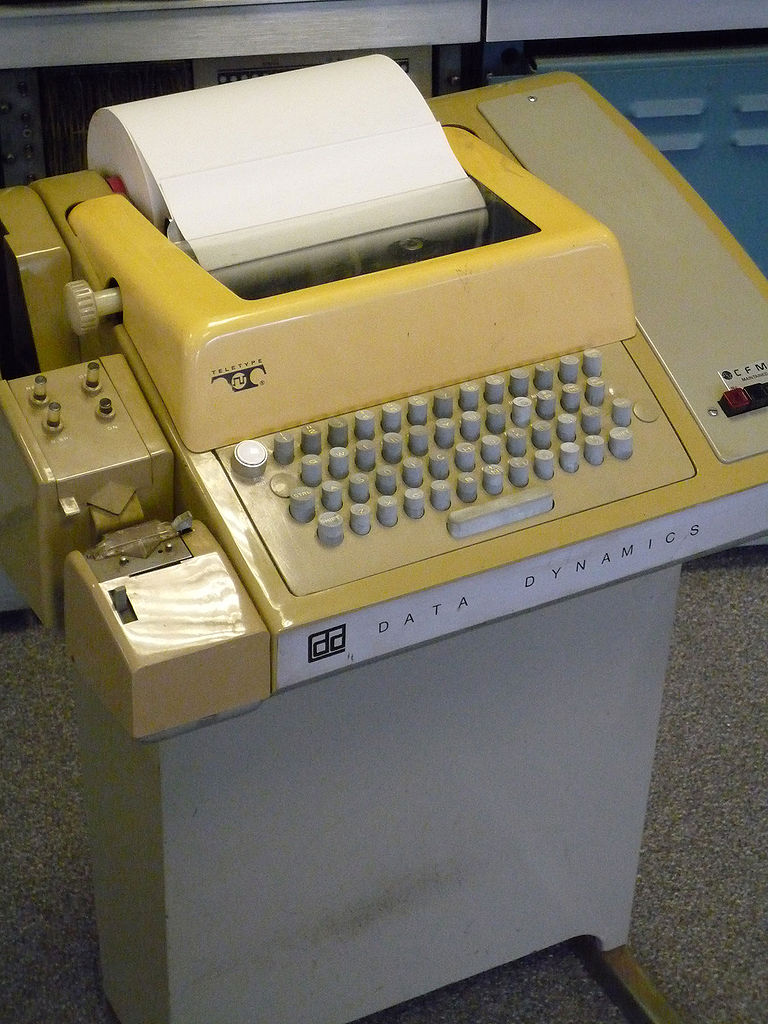
\includegraphics [width=\linewidth] {\inc/tty}
    \end {minipage}
    \hfill
    \begin {minipage} [c] {.68\linewidth}
	\begin {itemize}
	    \fB
	    \item il est relié par un lien série
		\begin {itemize}
		    \fC
		    \item paramètres : vitesse du lien, nombre
			de bits, parité
		    \item raccrocher le modem en fin de connexion
		    \item etc.
		\end {itemize}
	    \item il a des caractéristiques propres
		\begin {itemize}
		    \fC
		    \item caractères d'effacement, d'arrêt, de
			suspension, de fin de fichier, etc
		    \item bufferiser les caractères par ligne ou les
			envoyer sans attendre
		    \item nombre de lignes, de colonnes
		    \item etc.

		\end {itemize}
	\end {itemize}
    \end {minipage}

    \vspace* {2mm}

    \implique commande \code {stty} pour changer les paramètres (\implique
    \code {ioctl})

\end {frame}

\begin {frame} {Mode caractère}
    Un exemple particulier : le terminal (télétype)

    \begin {itemize}
	\fB
	\item le pilote a pour mission d'acheminer les octets
	    jusqu'au terminal

	\item certains programmes (ex: \code {zsh}, \code {vi},
	    \code {more}, etc.) doivent pouvoir en plus effacer l'écran,
	    positionner le curseur à un certain endroit, reconnaître
	    les touches de fonction, etc.

	\item séquences de contrôle différentes suivant les terminaux
	\item positionner le curseur à la ligne X et colonne Y : il faut envoyer...
	    \begin {itemize}
		\fD
		\item \framebox {ESC} \framebox {[} X \framebox {;}
		    Y \framebox {f} pour un terminal DEC VT100

		\item \framebox {ESC} \framebox {\&} \framebox {a}
		    Y \framebox {c} X \framebox {Y} pour un terminal
		    HP 2645

		\item Note : \framebox {ESC} = l'octet de code 27
	    \end {itemize}

	\item base \code {termcap}, puis \code {terminfo} pour l'ensemble
	    des séquences
	    \begin {itemize}
		\item variable d'environnement \code {TERM} : indique
		    le type de terminal
	    \end {itemize}

	\item les programmes (\code {zsh}, \code {vi}, etc.) doivent
	    utiliser cette base
	    \\
	    \implique ce n'est pas la mission du pilote

    \end {itemize}
\end {frame}

\begin {frame} {Mode caractère}
    Même principe pour la plupart des périphériques :

    \begin {itemize}
	\item le pilote achemine les octets jusqu'au périphérique
	\item ceci ne dispense pas les applications de gérer le
	    protocole de chaque périphérique

	    \begin {itemize}
		\item plusieurs protocoles différents pour les souris \\
		    \implique seul le serveur X-Window doit les connaître
		\item chaque imprimante dispose de son « langage de
		    contrôle »
		    \\
		    \implique tout programme souhaitant imprimer doit
		    disposer d'une collection d'adaptateurs pour les
		    différentes imprimantes (parfois nommés à tort
		    « pilotes »)
		\item etc.

	    \end {itemize}
    \end {itemize}
\end {frame}

\begin {frame} {Mode bloc}
    Interface du pilote :
    \begin {itemize}
	\item fonctions \code {open}, \code {close} : appelées au
	    montage/démontage du système de fichiers dans l'arborescence
	\item traitement d'interruption : idem mode brut
	\item fonction \code {strategy} : 2 rôles
	    \begin {itemize}
		\item lit un bloc en mémoire, dans le «~\textit {buffer
		    cache}~» (plus tard)
		\item écrit un bloc modifié du «~\textit {buffer cache}~»
		    vers le disque
		\item permet d'implémenter des optimisations \\
		    (ex : algorithme de l'ascenseur)
	    \end {itemize}
    \end {itemize}

    \vspace* {2mm}

    Note : la plupart des pilotes en mode bloc sont également
    accompagnés d'un pilote en mode caractère (pour \code {ioctl})
\end {frame}

\begin {frame} {Pseudo-périphériques}
    Un pilote peut offrir un service accessible via \code {read}
    ou \code {write} sans qu'il y ait un vrai périphérique

    \vspace* {3mm}

    Exemples :

    \ctableau {\fB} {|l|l|} {
	\rca \code {/dev/null} & poubelle \\
	\rcb \code {/dev/mem} & toute la mémoire de l'ordinateur \\
	\rca \code {/dev/random} & source d'aléa \\
    }

\end {frame}

\begin {frame} {Pseudo-périphériques}
    Cas particulier : les pseudo-terminaux

    \begin {itemize}
	\item beaucoup de programmes sont conçus pour être connectés
	    à un terminal

	\item comment fait \code {vi} lorsqu'on est connecté via
	    \code {ssh} ou via un terminal X-Window ?
	    \\
	    \implique il faut simuler un terminal et un lien série

	\item abstraction : pseudo-terminal

	    \begin {itemize}
		\item paire de pseudo-périphériques : maître et esclave
		\item gérés par le même pilote
		\item le serveur ssh gère le maître
		\item les programmes de la session accèdent
		    à l'esclave : il simule un « vrai » terminal
	    \end {itemize}
    \end {itemize}
\end {frame}

\begin {frame} {Pseudo-périphériques}

    \begin {minipage} [c] {.40\linewidth}
	\includegraphics [width=\linewidth] {\inc/pty}
    \end {minipage}
    \hfill
    \begin {minipage} [c] {.58\linewidth}
	\begin {itemize}
	    \fB
	    \item le serveur ssh ouvre la paire
	    \item tout octet émis vers le maître (resp. esclave)
		est transmis vers l'esclave (resp. maître)
	    \item le serveur ssh transmet les octets reçus depuis
		le réseau vers le maître
	    \item les programmes de la session ssh (\code {sh},
		\code {vi}) sont connectés à l'esclave
	    \item tout changement de paramètre terminal (via \code {ioctl})
		est transmis au serveur ssh
	\end {itemize}
    \end {minipage}

    \begin {itemize}
	\item autres utilisations :
	    \begin {itemize}
		\item fenêtres « terminal » en environnement graphique
		\item \code {script} (enregistrement de session)
		\item programmes \code {screen} et \code {tmux}
	    \end {itemize}
    \end {itemize}

\end {frame}

\begin {frame} {Évolutions}
    Réalité : malheureusement très complexe...
    \begin {center}
	\includegraphics [width=.6\linewidth] {\inc/arch-now}
    \end {center}

    Exemple : disques connectés via le bus SATA, SCSI,
    USB ou même via un ancestral bus IDE.

\end {frame}

\begin {frame} {Évolutions}
    \begin {itemize}
	\item complexité matérielle accrue

	    \begin {itemize}
		\item gestion des différents niveaux de bus
		\item partage de code entre pilotes (exemple : disques)
	    \end {itemize}

	\item dynamicité des périphériques

	    \begin {itemize}
		\item connecter ou déconnecter des périphériques « à chaud »
		\item auto-reconnaissance des périphériques
	    \end {itemize}
    \end {itemize}

    \implique complexité des pilotes
\end {frame}


%%%%%%%%%%%%%%%%%%%%%%%%%%%%%%%%%%%%%%%%%%%%%%%%%%%%%%%%%%%%%%%%%%%%%%%%%%%%%%
% Le répertoire /dev
%%%%%%%%%%%%%%%%%%%%%%%%%%%%%%%%%%%%%%%%%%%%%%%%%%%%%%%%%%%%%%%%%%%%%%%%%%%%%%

\titreB {Le répertoire /dev}

\begin {frame} {Le répertoire /dev}
    Historiquement, le répertoire \code {/dev} était peuplé «~à
    la main~»

    \begin {itemize}
	\item peu d'ajout ou de suppression de périphériques
	\item commande \code {mknod}
	\item script \code {MAKEDEV} dans \code {/dev}
    \end {itemize}
\end {frame}

\begin {frame} {Le répertoire /dev}
    Évolution \implique ajout dynamique de périphériques

    \begin {itemize}

	\item Système de fichier « devfs »

	    \begin {itemize}
		\item création/destruction automatique des fichiers spéciaux
		\item nécessite des périphériques capables de s'identifier
		    \begin {itemize}
			\item « plug and play »
		    \end {itemize}
	    \end {itemize}

	\item Programme additionnel pour gérer les exceptions

	    \begin {itemize}
		\item je veux un lien \code {/dev/cédérom} vers le
		    troisième lecteur de CD de mon système

		\item je veux pouvoir connecter mon appareil photo
		    sans avoir les droits de l'administrateur
	    \end {itemize}
    \end {itemize}
\end {frame}

\def\inc{inc4-ps}

\titreA {Gestion des processus}

%%%%%%%%%%%%%%%%%%%%%%%%%%%%%%%%%%%%%%%%%%%%%%%%%%%%%%%%%%%%%%%%%%%%%%%%%%%%%%
% Introduction
%%%%%%%%%%%%%%%%%%%%%%%%%%%%%%%%%%%%%%%%%%%%%%%%%%%%%%%%%%%%%%%%%%%%%%%%%%%%%%

\titreB {Introduction}

\begin {frame} {Définition d'un processus (haut niveau)}
    Définition (haut niveau) :

    \begin {quote}
	un processus est une instance d'un programme en cours d'exécution
    \end {quote}

    ... mais pas n'importe quelle exécution :

    \begin {itemize}
	\item j'exécute \code {ls /tmp} : le processus correspond à
	    l'exécution du programme \code {ls} avec les données
	    \code {/tmp}

	\item quelqu'un d'autre exécute \code {ls /tmp} en même
	    temps : ce n'est pas la même exécution, même si c'est le
	    même programme et les mêmes données

	    \begin {itemize}
		\item ce n'est pas le même processus
		\item même si le « quelqu'un d'autre », c'est moi
	    \end {itemize}

    \end {itemize}
\end {frame}

\begin {frame} {Attributs d'un processus}
    Un processus possède des attributs :

    \begin {itemize}
	\fB
	\item état (prêt à tourner, en attente, etc.)
	\item identificateur de processus (pid)
	\item identificateur de processus parent (ppid)
	\item propriétaire (uid), groupe (gid)
	\item ouvertures de fichiers
	\item répertoire courant
	\item terminal de contrôle
	\item localisation en mémoire
	\item consommation de temps CPU
	\item etc.
    \end {itemize}

\end {frame}

\begin {frame} {Définition d'un processus (bas niveau)}
    Définition (bas niveau) :

    \begin {quote}
	un processus est décrit par :
	\begin {itemize}
	    \fB
	    \item un espace mémoire pour le programme et les données
	    \item des attributs
	    \item un contexte matériel
		\begin {itemize}
		    \fC
		    \item registres du processeur
		    \item traduction d'adresses
		\end {itemize}
	\end {itemize}
    \end {quote}

    { \fB (voir \code {task\_struct} sur
	\url {http://www.tldp.org/LDP/tlk/ds/ds.html} )}

    \vspace* {2mm}

    À chaque fois :
    \begin {itemize}
	\fB
	\item qu'un processus est retiré du processeur
	    \begin {itemize}
		\fC
		\item son contexte est sauvegardé (espace mémoire, registres
		    du processeur, etc.)
	    \end {itemize}
	\item qu'un processus est mis sur le processeur
	    \begin {itemize}
		\fC
		\item son contexte est restauré
	    \end {itemize}
    \end {itemize}
\end {frame}

\begin {frame} {Espace mémoire d'un processus}
    Découpage en 3 zones :

    \begin {minipage} [c] {.29\linewidth}
	\includegraphics [width=\linewidth] {\inc/segments}
    \end {minipage}
    \hfill
    \begin {minipage} [c] {.69\linewidth}
	\begin {itemize}
	    \fB
	    \item segment « text »
		\begin {itemize}
		    \fC
		    \item programme (code compilé)
		    \item adresse 0 pas utilisée : pourquoi ?
		\end {itemize}
	    \item segment « data »
		\begin {itemize}
		    \fC
		    \item variables globales (+ \code {static} locales)
		    \item tas (mémoire allouée par \code {malloc})
		    \item extension explicite (via \code {malloc})
		\end {itemize}
	    \item segment « stack » : la pile d'exécution
		\begin {itemize}
		    \fC
		    \item variables locales
		    \item arguments des fonctions
		    \item adresses de retour
		    \item extension implicite (utilisation de la pile)
		\end {itemize}
	    \item d'autres zones peuvent être ajoutées
		\begin {itemize}
		    \fC
		    \item bibliothèques partagées
		    \item mémoire partagée entre processus
		    \item \implique cf semestre 5
		\end {itemize}
	\end {itemize}
    \end {minipage}

\end {frame}

%%%%%%%%%%%%%%%%%%%%%%%%%%%%%%%%%%%%%%%%%%%%%%%%%%%%%%%%%%%%%%%%%%%%%%%%%%%%%%
% Gestion des attributs
%%%%%%%%%%%%%%%%%%%%%%%%%%%%%%%%%%%%%%%%%%%%%%%%%%%%%%%%%%%%%%%%%%%%%%%%%%%%%%

\titreB {Gestion des attributs}

\begin {frame} {Identité}
    \prototype {
	\code {pid\_t getpid (void)} 
	\hspace* {10mm}
	\code {pid\_t getppid (void)} \\
	\code {uid\_t getuid (void)}
	\hspace* {10mm}
	\code {gid\_t getgid (void)}
    }

    \begin {itemize}
	\item Primitives simples...
	\item Ne renvoient pas -1 en cas d'erreur (pas d'erreur possible)
	\item Exemple :
	    \lstinputlisting [basicstyle=\fD\lstmonstyle] {\inc/getpid.c}
    \end {itemize}
\end {frame}

\begin {frame} {Identité}
    \prototype {
	\code {int setuid (uid\_t uid)}
	\hspace* {10mm}
	\code {int setgid (gid\_t gid)}
    }

    \begin {itemize}
	\item Primitives restreintes à l'administrateur (uid = 0)

	\item Utilisées lors de l'admission sur le système :
	    \begin {itemize}
		\item \code {/bin/login}, \code {sshd} ou équivalent pour
		    X-Window
		\item lancé par le processus numéro 1 ou un de ses
		    descendants
	    \end {itemize}
    \end {itemize}
\end {frame}

\begin {frame} {Identité}

    Algorithme de l'admission sur le système :
    \begin {enumerate}
	\item demander login et mot de passe
	\item chercher l'entrée dans \code {/etc/passwd}
	    \begin {itemize}
		\item lignes de la forme : \\
		    {\fD \code {toto:sel+mot-de-passe-chiffré:uid:gid:nom:répertoire:shell}}
		\item sel et mot de passe chiffré sont mis dans
		    un fichier séparé (\code {/etc/shadow} sur Linux)
	    \end {itemize}
	\item chiffrer le mot de passe (avec le « sel » cité
	    dans l'entrée)
	\item comparer le mot de passe avec l'entrée
	\item si identique
	    \begin {itemize}
		\item générer un nouveau processus
		\item \code {setuid (uid)} / \code {setgid (gid)}
		    dans ce nouveau processus
		\item lancer l'exécution du shell (ou du
		    «~window manager~»)
	    \end {itemize}
    \end {enumerate}
\end {frame}

\begin {frame} {Masque de création de fichiers}
    \prototype {
	\code {mode\_t umask (mode\_t masque)}
    }

    \begin {itemize}
	\item Création de fichier (\code {open (}... \code
	    {O\_CREAT}...\code {)}, \code {mkdir} ou \code {mknod})

	    \begin {itemize}
		\item permissions du fichier créé = mode \code {\& \~{}} umask
		\begin {center}
		    \includegraphics [width=.7\linewidth] {\inc/umask}
		\end {center}
	    \end {itemize}

	\item Recommandation : dans les programmes \implique 0666 ou 0777
	    \begin {itemize}
		\item les programmes sont généraux
		\item laisser l'utilisateur gérer son niveau de confidentialité
		    \begin {itemize}
			\item commande \code {umask} du Shell
		    \end {itemize}
		\item sauf pour les programmes sensibles à la sécurité
	    \end {itemize}

	\item \code {umask} renvoie l'ancien masque (avant modification)

    \end {itemize}
\end {frame}

\begin {frame} {Répertoire courant}
    \prototype {
	\code {int chdir (const char *path)}
    }

    \begin {itemize}
	\item Modifie le répertoire courant du processus
	\item Rappel : le répertoire courant est un attribut du processus
	    \begin {itemize}
		\item changer dans un processus n'affecte pas les autres
		    processus
	    \end {itemize}

	\item Pas de primitive système pour récupérer le nom
	    du répertoire courant

	    \begin {itemize}
		\item c'est une fonction de bibliothèque
		    \prototype {
			\code {char *getcwd (char *buf, size\_t max)}
		    }
		\item comment fonctionne-t'elle ?
	    \end {itemize}

    \end {itemize}
\end {frame}

\begin {frame} {Racine courante}
    \prototype {
	\code {int chroot (const char *path)}
    }

    \begin {itemize}
	\item Modifie la racine courante du processus
		\begin {center}
		    \includegraphics [width=.9\linewidth] {\inc/chroot}
		\end {center}

	\item Pas de possibilité de contournement
	    \begin {itemize}
		\item à la nouvelle racine, «~\code {..}~» reste au
		    même endroit
		\item on ne peut que descendre dans l'arborescence
	    \end {itemize}
	\item Accessible seulement à l'administrateur du système
	\item Primitive non normalisée par POSIX
    \end {itemize}
\end {frame}

\begin {frame} {Racine courante}
    \code {chroot} est un système de confinement :

    \begin {itemize}
	\item restreindre l'environnement à certains fichiers
	    seulement
	    \begin {itemize}
		\item exemple : comptes utilisateurs spécifiques
		    pour accéder à une application seulement
		\item exemple : serveur « FTP anonyme » \\
		    service FTP pour distribuer des fichiers, restreint
		    à une portion de l'arborescence

	    \end {itemize}

	\item \code {chroot} : base des systèmes de « conteneurs » modernes
		\begin {itemize}
		    \item LXC sur Linux, Jails sur FreeBSD
		    \item complété par d'autres systèmes de confinement
			\begin {itemize}
			    \item visibilité restreinte des processus
			    \item visibilité restreinte des connexions réseau
			    \item etc.
			\end {itemize}
		    \item machines « virtuelles » à moindre coût
		\end {itemize}

    \end {itemize}
\end {frame}

%%%%%%%%%%%%%%%%%%%%%%%%%%%%%%%%%%%%%%%%%%%%%%%%%%%%%%%%%%%%%%%%%%%%%%%%%%%%%%
% Création des processus
%%%%%%%%%%%%%%%%%%%%%%%%%%%%%%%%%%%%%%%%%%%%%%%%%%%%%%%%%%%%%%%%%%%%%%%%%%%%%%

\titreB {Création des processus}

\begin {frame} {Création des processus}
    \prototype {
	\code {pid\_t fork (void)}
    }

    Créer un processus $\Longleftrightarrow$ dupliquer le processus

    \begin {itemize}
	\item Primitive \code {fork} = photocopieuse à processus
	\item Processus = mémoire + attributs + contexte matériel
	    \begin {itemize}
		\item (presque) tout est dupliqué
		\item mémoire dupliquée \implique variables dupliquées
		\item les registres du CPU aussi : chaque programme
		    évoluera (registre PC) séparément
	    \end {itemize}
	\item Duplication \implique informations \textbf {héritées}
	    du processus père
	    \begin {itemize}
		\item répertoire courant, ouvertures de fichiers, etc.
		\item sauf quelques attributs~: pid, ppid, temps CPU, etc.
	    \end {itemize}
	\item Après une photocopie, on peut écrire sur chaque feuille
	    de papier, ça ne modifie pas l'autre feuille
	    \begin {itemize}
		\item c'est la même chose avec \code {fork}
	    \end {itemize}
    \end {itemize}
\end {frame}

\begin {frame} {Création des processus}
    \begin {minipage} [c] {.30\linewidth}
	\lstinputlisting [basicstyle=\fE\lstmonstyle] {\inc/fork.c}
    \end {minipage}
    \hfill
    \begin {minipage} [c] {.69\linewidth}
	\includegraphics [width=1.1\linewidth] {\inc/fork}
    \end {minipage}

    \vspace* {3mm}

    Après \code {fork} : les variables \code {x} et \code {pid}
    évoluent séparément
\end {frame}

\begin {frame} {Création des processus}
    \begin {itemize}
	\item Particularité de \code {fork} :
	    \begin {itemize}
		\item un seul appel, deux retours
		    \begin {itemize}
			\item comme \code {fork} duplique le processus,
			    tout se passe pour le deuxième comme s'il
			    avait lui-même appelé \code {fork}
		    \end {itemize}

	    \end {itemize}
	\item Valeur de retour de \code {fork} :
	    \begin {itemize}
		\item -1 en cas d'erreur (classique)
		\item 0 pour le processus fils
		\item une valeur > 0 pour le processus père
		    \begin {itemize}
			\item c'est le pid du fils
		    \end {itemize}
	    \end {itemize}
	\item Pas de déterminisme :
	    \begin {itemize}
		\item après \code {fork}, on ne sait pas si le père ou
		    le fils est remis sur le processeur en premier
		\item pas un problème : les processus évoluent indépendamment
	    \end {itemize}
    \end {itemize}
\end {frame}

\begin {frame} {Création des processus}
    \begin {itemize}
	\item Quel moyen mnémotechnique pour la valeur de retour ?
	    \begin {itemize}
		\item Chaque processus connaît son père
		    \begin {itemize}
			\item attribut ppid, primitive \code {getpid}
			\item information facile à retrouver
			\item \implique pas besoin de récupérer
			    le pid du père avec \code {fork}
			\item \code {fork} renvoie donc 0 pour le fils
		    \end {itemize}

		\item Pas de moyen facile pour récupérer le pid du fils
		    \begin {itemize}
			\item il peut y en avoir beaucoup, lequel renvoyer ?
			\item pas d'attribut, pas de primitive
			\item \implique seul moyen de récupérer le pid du
			    fils = \code {fork}
			\item \code {fork} renvoie au père le pid du fils
		    \end {itemize}
	    \end {itemize}
    \end {itemize}
\end {frame}

\begin {frame} {Création des processus}
    Quelques conseils pour apprivoiser \code {fork} :

    \begin {itemize}
	\item \code {switch} avec 3 cas : \code {-1}, \code {0} et
	    \code {default}

	    \begin {itemize}
		\item pour être sûr de n'oublier aucun cas
	    \end {itemize}
	\item dans le cas 0 (fils), faire appel à une fonction \code {fils}
	    et terminer par \code {exit}
	    \begin {itemize}
		\item isoler le code du fils
		\item placer un « cordon sanitaire » afin que le fils
		    n'exécute pas le code prévu pour le père
	    \end {itemize}
    \end {itemize}
\end {frame}

\begin {frame} {Création des processus}
    Exemple :

    \lstinputlisting [basicstyle=\fC\lstmonstyle] {\inc/ex-fork.c}
\end {frame}

\begin {frame} {Terminaison des processus}
    \prototype {
	\code {void exit (int code)}
    }

    \begin {itemize}
	\item Termine le processus en cours
	\item Pas de retour (et pas -1 en cas d'erreur)
	\item Presque toutes les ressources sont libérées
	    \begin {itemize}
		\item mémoire, CPU, etc.
		\item cas particulier pour les processus zombies (plus tard)
	    \end {itemize}
	\item Argument \code {code} $\in$ [0..255]
	    \begin {itemize}
		\item si vous voyez \code {\alert {exit (-1)}} dans un
		    programme, c'est que son auteur n'a pas assimilé
		    son cours de système...
		\item valeur 0 : ok (pour le Shell)
		\item constantes POSIX : \code {EXIT\_SUCCESS} et \code
		    {EXIT\_FAILURE}

	    \end {itemize}
	\item En réalité, \code {exit} est une fonction de bibliothèque
	    \begin {itemize}
		\item vide les buffers des fichiers ouverts par \code {fopen}
		\item appelle les fonctions enregistrées par \code {atexit}
		\item la vraie primitive s'appelle \code {\_exit}
		    \begin {itemize}
			\item jamais appelée directement
		    \end {itemize}
	    \end {itemize}
    \end {itemize}
\end {frame}

\begin {frame} {Terminaison des processus}
    \prototype {
	\code {pid\_t wait (int *raison)} \\
	\code {pid\_t waitpid (pid\_t pid, int *raison, int options)} \\
    }

    \vspace* {-8mm}

    \begin {itemize}
	\item Attend la terminaison d'un des processus fils
	    \begin {itemize}
		\item \code {wait} attend n'importe quel fils
		    \begin {itemize}
			\item si un processus fils est déjà terminé,
			    pas d'attente
			\item si pas de processus fils, renvoie -1
			\item s'il y a au moins un processus fils, attente
			\item si attente interrompue par un signa, renvoie -1
		    \end {itemize}
		\item \code {waitpid} attend un processus spécifique
		    (voir manuel)
	    \end {itemize}
	\item La terminaison peut avoir plusieurs causes :
	    \begin {itemize}
		\item le fils appelle \code {exit}
		\item le fils reçoit un signal
		    \begin {itemize}
			\item \framebox {\fD CTRL} \framebox {\fD C}, violation
			    de segment, etc.
		    \end {itemize}
		\item ce peut être autre chose qu'une terminaison
		    \begin {itemize}
			\item processus ayant atteint un point d'arrêt avec
			    un débogueur
		    \end {itemize}

	    \end {itemize}
    \end {itemize}
\end {frame}

\begin {frame} {Terminaison des processus}
    \begin {itemize}
	\item Entier pointé par \code {raison} : raison de la terminaison
	    \ctableau {\fE} {|p{.2\linewidth}|p{.2\linewidth}|p{.2\linewidth}|p{.2\linewidth}|} {
		\rca \multicolumn {1}{|c|}{\textbf {}} & 
		    \multicolumn {1}{c|}{\textbf {code retour}} &
		    \multicolumn {1}{c|}{\textbf {poids fort}} &
		    \multicolumn {1}{c|}{\textbf {poids faible}}
		    \\
		\rcb processus stoppé en mode trace &
		    identificateur~du pro\-ces\-sus &
		    numéro du signal &
		    \multicolumn {1}{c|}{0177}
		    \\
		\rca processus terminé par exit &
		    identificateur~du pro\-ces\-sus &
		    argument de exit sur 8 bits &
		    \multicolumn {1}{c|}{0}
		    \\
		\rcb processus terminé par signal &
		    identificateur~du pro\-ces\-sus &
		    \multicolumn {1}{c|}{0} &
		    numéro du signal (+0200 si core)
		    \\
		\rca wait interrompue par signal &
		    \multicolumn {1}{c|}{-1} &
		    \multicolumn {1}{c|}{?} &
		    \multicolumn {1}{c|}{?}
		    \\
	    }
	    \vspace* {3mm}

	\item POSIX simplifie le travail : macros les plus courantes

	    \ctableau {\fC} {|l|l|} {
		\rca Arrêt avec \code {exit} ? & WIFEXITED () \\
		\rcb \implique si oui, code de retour & WEXITSTATUS () \\
		\rca Arrêt sur signal ? & WIFSIGNALED () \\
		\rcb \implique si oui, numéro du signal & WTERMSIG () \\
	    }
    \end {itemize}
\end {frame}

\begin {frame} {Terminaison des processus}
    Exemple :

    \lstinputlisting [basicstyle=\fD\lstmonstyle] {\inc/ex-wait.c}
\end {frame}

\begin {frame} {Cas particulier -- Processus zombie}
    Définition :

    \begin {quote}
	Un processus zombie est un processus terminé, dont le
	père n'a pas encore enregistré la terminaison avec wait
    \end {quote}

    \begin {itemize}
	\item un processus zombie est « quasiment » terminé
	    \begin {itemize}
		\item presque toutes ses ressources sont libérées...
		\item ... sauf le descripteur du processus
		    \begin {itemize}
			\item il contient la raison de la terminaison
			\item ainsi qu'un résumé de l'utilisation
			    des ressources
		    \end {itemize}
		\item sans limitation de durée
		\item il reste visible avec \code {ps}
	    \end {itemize}


	\item lorsque le père utilise \code {wait} :

	    \begin {itemize}
		\item il collecte les informations nécessaires
		\item le descripteur de processus est libéré
		    \begin {itemize}
			\item le processus disparaît alors complètement
			    du système
		    \end {itemize}

	    \end {itemize}
    \end {itemize}
\end {frame}

\begin {frame} {Cas particulier -- Processus orphelin}
    Que se passe-t'il lorsque le père d'un processus se termine ?

    \vspace* {2mm}

    \begin {minipage} [c] {.24\linewidth}
	\includegraphics [width=\linewidth] {\inc/orphan}
    \end {minipage}
    \hfill
    \begin {minipage} [c] {.75\linewidth}
	\begin {itemize}
	    \item père se termine \implique zombie
	    \item dès que le père devient zombie, le fils est «~reparenté~»
		    (ppid $\leftarrow$ 1)
	    \item le processus 1 est spécial
		\begin {itemize}
		    \item ne s'arrête jamais
		    \item (re-)démarre les programmes du système
		    \item algorithme :
			\lstinputlisting [basicstyle=\fE\lstmonstyle] {\inc/algo-ps1.c}
		\end {itemize}
	\end {itemize}
    \end {minipage}

    \vspace* {2mm}

    \implique le fils est immédiatement reparenté \\
    \implique le statut d'orphelin n'existe donc pas dans le noyau
\end {frame}

\begin {frame} {États d'un processus}
    États d'un processus :
    \begin {center}
	\includegraphics [width=.8\linewidth] {\inc/etats}
    \end {center}
\end {frame}


%%%%%%%%%%%%%%%%%%%%%%%%%%%%%%%%%%%%%%%%%%%%%%%%%%%%%%%%%%%%%%%%%%%%%%%%%%%%%%
% Exécution d'un fichier
%%%%%%%%%%%%%%%%%%%%%%%%%%%%%%%%%%%%%%%%%%%%%%%%%%%%%%%%%%%%%%%%%%%%%%%%%%%%%%

\titreB {Exécution d'un fichier}

\begin {frame} {Exécution d'un fichier}
    \prototype {
	\fC \code {int execl (char *path, char *arg, ... )} \\
	\fC \code {int execv (char *path, char *argv [])} \\
	\fC \code {int execle (char *path, char *arg, ..., char *envp [])} \\
	\fC \code {int execve (char *path, char *argv [], char *envp [])} \\
	\fC \code {int execlp (char *fichier, char *arg0, ...)} \\
	\fC \code {int execvp (char *fichier, char *argv [])}
    }

    \begin {itemize}
	\item Primitives \code {exec*} : remplacent le programme du
	    processus courant par un nouveau programme et ses arguments

	    \begin {itemize}
		\item le contexte du processus reste quasiment inchangé
		    \begin {itemize}
			\item attributs inchangés : pid, ppid, uid
			    (sauf exception), umask, répertoire courant,
			    consommation de ressources, etc.

			\item attributs modifiés : référence à l'exécutable,
			    ouvertures de fichiers (sauf exception, notamment
			    pour 0, 1 et 2), etc.
		    \end {itemize}
		\item mémoire initialisée avec le nouveau programme
		    \begin {itemize}
			\item segments text, data et stack
		    \end {itemize}
	    \end {itemize}
	\item Valeur de retour = -1 (toujours)
	    \begin {itemize}
		\item retour \implique nouveau programme non chargé
		    \implique erreur
	    \end {itemize}
    \end {itemize}
\end {frame}

\begin {frame} {Exécution d'un fichier}
    \begin {center}
	\includegraphics [width=.8\linewidth] {\inc/exec}
    \end {center}
\end {frame}

\begin {frame} {Exécution d'un fichier -- Exemple}
    Pas de retour pour \code {exec*} \implique le plus souvent utilisée
    avec \code {fork}

    \vspace* {3mm}

    \lstinputlisting [basicstyle=\fD\lstmonstyle] {\inc/ex-exec.c}
\end {frame}

\begin {frame} {Exécution d'un fichier -- Exemple}
    Autre exemple : algorithme (grossier) du Shell

    \begin {enumerate}
	\item lire une ligne
	\item découper la ligne en éléments
	\item si éléments [0] $\in$ commandes internes
	    \begin {itemize}
		\item alors exécuter la fonction correspondante
		\item revenir en 1
	    \end {itemize}
	\item localiser le fichier éléments [0] dans \code {PATH}
	\item si pas trouvé, alors erreur et revenir en 1
	\item \code {fork} \implique fils
	    \begin {itemize}
		\item \code {exec (} éléments \code {)}
	    \end {itemize}
	\item si éléments [end] $\neq$ \code {\&}
	    \begin {itemize}
		\item alors attendre la fin du fils
	    \end {itemize}
	\item revenir en 1
    \end {enumerate}
\end {frame}

\begin {frame} {Exécution d'un fichier -- Environnement}
    En plus des arguments, \code {exec*} passe l'environnement :

    \vspace* {4mm}

    \begin {minipage} [c] {.35\linewidth}
	\includegraphics [width=1.2\linewidth] {\inc/env}
    \end {minipage}
    \hfill
    \begin {minipage} [c] {.64\linewidth}
	\begin {itemize}
	    \item \code {extern char **environ}
	    \item fonction de bibliothèque \code {getenv}
	    \item environnement modifié par le Shell
		\begin {itemize}
		    \item hérité par tous les processus lancés
			par le Shell
		    \item rappel : utiliser \code {export} en Shell pour
			exporter une variable d'environnement

		\end {itemize}
	\end {itemize}
    \end {minipage}
\end {frame}

\begin {frame} {Exécution d'un fichier}
    Six formes pour \code {exec*} :

    \begin {itemize}
	\item passage des arguments :
	    \ctableau {\fC} {|l|l|} {
		\rca \code {execl}
		    & en liste : \code {execl (..., "echo", "a, "b", NULL)} \\
		\rcb \code {execl}
		    & en vecteur : \code {execv (..., tabargv)} \\
	    }

	    \vspace* {2mm}

	\item recherche dans la variable shell \code {PATH} :
	    \ctableau {\fC} {|l|l|} {
		\rca \code {exec[vl]}
		    & non : \code {execv ("/bin/echo", tabargv)} \\
		\rcb \code {exec[vl]p}
		    & oui : \code {execvp ("echo", tabargv)} \\
	    }

	    \vspace* {2mm}

	\item passage de l'environnement :

	    \ctableau {\fC} {|l|l|} {
		\rca \code {exec[vl]}
		    & implicite : \code {execv ("/bin/echo", tabargv)} \\
		\rcb \code {exec[vl]e}
		    & explicite : \code {execve ("echo", tabargv, tabenvp)} \\
	    }

    \end {itemize}

    \vspace* {2mm}

    Une seule de ces formes est une primitive système (laquelle ?) \\
    \implique les autres sont des fonctions de bibliothèque
\end {frame}

\begin {frame} {Nombres magiques}
    \code {exec*} peut exécuter plusieurs sortes de fichiers :

    \begin {itemize}
	\item Fichiers binaires (compilés)
	    \begin {itemize}
		\item plusieurs formats possibles
		    \begin {itemize}
			\item évolution des formats,
			    compatibilité avec anciennes versions
			\item sur FreeBSD : mode de compatibilité Linux
		    \end {itemize}
	    \end {itemize}
	\item Fichiers interprétés
	    \begin {itemize}
		\item fichiers non directement exécutables
		    \begin {itemize}
			\item recours à un interprète
			\item Shell, Awk, Perl, Tcl, Ruby, Python, etc.
		    \end {itemize}
		\item l'interprète ouvre le fichier et l'« exécute »
	    \end {itemize}
    \end {itemize}

    \vspace* {1mm}

    Présence d'un « nombre magique » en début de fichier

    \ctableau {\fC} {|l|l|} {
	\rca fichiers binaires
	    & \code {0x7f 'E' 'L' 'F'} (format ELF sous Linux) \\
	\rcb fichiers interprétés
	    &  \code {'\#' '!'} (suivi du chemin de l'interprète) \\
    }

\end {frame}

%%%%%%%%%%%%%%%%%%%%%%%%%%%%%%%%%%%%%%%%%%%%%%%%%%%%%%%%%%%%%%%%%%%%%%%%%%%%%%
% Droits d'exécution
%%%%%%%%%%%%%%%%%%%%%%%%%%%%%%%%%%%%%%%%%%%%%%%%%%%%%%%%%%%%%%%%%%%%%%%%%%%%%%

\titreB {Droits d'exécution}

\begin {frame} {Droits d'exécution}
    \begin {center}
	\includegraphics [width=.8\linewidth] {\inc/droits}
    \end {center}

    \begin {itemize}
	\item \code {fork} : le fils hérite de l'uid (celui de tata)
	\item \code {exec} : ne change pas l'uid (celui de tata)
	\item le fichier \code {secret.txt} de l'utilisateur toto
	    ne peut pas être ouvert par un processus appartenant à tata
	\item \implique le système de droits fonctionne bien !

    \end {itemize}
\end {frame}

\begin {frame} {Droits d'exécution -- Élévation de privilège}
    Dans certains cas, il faut pouvoir exécuter un programme avec
    des droits plus élevés :

    \begin {itemize}
	\item un utilisateur change son mot de passe \implique
	    il doit écrire le nouveau mot de passe chiffré dans \code
	    {/etc/passwd}

	    \begin {itemize}
		\fC
		\item \code {/etc/paswd} n'est pas modifiable par
		    l'utilisateur \\
		    \fC
		    \code {\$ ls -l /etc/passwd} \\
		    \code {-rw-r--r-- 1 root 12345 Jan 1  1970 /etc/passwd}

	    \end {itemize}

	\item un utilisateur insère la carte SD de son appareil photo \\
	    \implique
	    le système de fichiers sur la carte doit être « monté »

	    \begin {itemize}
		\fC
		\item l'opération de montage (primitive système \code
		    {mount}) n'est accessible qu'à l'administrateur
	    \end {itemize}

	\item un utilisateur souhaite utiliser la commande \code {ping}

	    \begin {itemize}
		\fC
		\item \code {ping} accède aux couches réseau de bas
		    niveau et nécessite les privilèges de 
		    l'administrateur 
	    \end {itemize}

    \end {itemize}
\end {frame}

\begin {frame} {Droits d'exécution -- Élévation de privilège}
    Retour sur les permissions de fichiers :

    \begin {center}
	\includegraphics [width=.7\linewidth] {\inc/perm}
    \end {center}

    \begin {itemize}
	\item bit «~\textit {set-user-id-on-exec}~» (ou bit «~suid~»)
	\item bit «~\textit {set-group-id-on-exec}~» (ou bit «~sgid~»)
    \end {itemize}
\end {frame}

\begin {frame} {Droits d'exécution -- Bit set-user-id-on-exec}

    \begin {itemize}
	\item Appel à \code {exec} : si le bit «~suid~» est à 1,
	    alors l'uid du processus devient l'uid du propriétaire
	    du fichier

	    \begin {itemize}
		\item autrement dit : commande exécutée avec
		    les droits du propriétaire (de la commande) et non
		    ceux de l'utilisateur

	    \end {itemize}

	\item Exemple :
	    \begin {itemize}
		\item la commande \code {/bin/passwd} appartient à root
		\item dans ses permissions, le bit «~suid~» est à 1
		\item \implique le processus peut donc modifier
		    \code {/etc/passwd}
		\item \implique l'utilisateur peut changer son mot de
		    passe !
	    \end {itemize}
    \end {itemize}
\end {frame}

\begin {frame} {Droits d'exécution -- Bit set-user-id-on-exec}

    \begin {itemize}
	\item Problème 1 : \code {/bin/passwd} doit connaître l'uid de
	    l'utilisateur qui change son mot de passe...
	    \\
	    \implique 2 notions d'uid distinctes :

	    \vspace* {-2mm}

	    \ctableau {\fC} {|l|l|l|} {
		\rca uid réel
		    & l'humain derrière son terminal
		    & \code {uid\_t getuid (void)}
		    \\
		\rcb uid effectif
		    & l'uid servant à tester les droits
		    & \code {uid\_t geteuid (void)}
		    \\
	    }
    \end {itemize}
\end {frame}

\begin {frame} {Droits d'exécution -- Bit set-user-id-on-exec}
    \begin {itemize}
	\item Problème 2 : pour certaines opérations, il faut utiliser
	    l'uid réel et non effectif
	    \begin {itemize}
		\item exemple : création de fichier
		    \implique propriétaire = uid effectif
		\item parfois, il repasser temporairement sous l'identité
		    de l'utilisateur réel
		    \begin {itemize} 
			\item exemple : pour créer le fichier sous la bonne identité
		    \end {itemize}

		\item d'où une troisième notion : uid « sauvé »
		    \begin {itemize}
			\item l'uid sauvé permet de sauver l'uid effectif
			    si jamais on le change (avec
			    \code {int seteuid (uid\_t euid)})
			\item permet de passer sous l'identité de
			    l'uid réel, puis de repasser à nouveau
			    sous l'identité privilégiée
		    \end {itemize}
	    \end {itemize}
    \end {itemize}
\end {frame}

\begin {frame} {Droits d'exécution -- Bit set-group-id-on-exec}
    Application des mêmes principes au groupe :

    \begin {itemize}
	\item bit «~set-group-id-on-exec~»
	\item 3 identités
	    \begin {itemize}
		\item gid réel
		\item gid effectif
		\item gid sauvé
	    \end {itemize}
    \end {itemize}

    \vspace* {5mm}
    Note :

    \begin {itemize}
	\item \code {ls} affiche ces bits
	\item exemple :

	    \vspace* {1mm}

	    {\fD
	    \code {\$ ls -l /usr/bin/passwd /usr/bin/crontab} \\
	    \code {-rw\alert {s}r-xr-x 1 root root\ \ \ \  12345 Jan 1  1970 /usr/bin/passwd} \\
	    \code {-rwxr-\alert {s}r-x 1 root crontab 23456 Jan 1  1970 /usr/bin/crontab}
	    }

    \end {itemize}
\end {frame}

\begin {frame} {Droits d'exécution -- Élévation de privilège}
    Bits «~suid~» et «~sgid~» : changent le niveau de privilège

    \begin {itemize}
	\item le plus souvent : pour élever le niveau
	    \begin {itemize}
		\item même si ça peut arriver de le diminuer
	    \end {itemize}

	\item ce sont des problèmes de sécurité potentiels

	    \begin {itemize}
		\item privilèges \implique attention à la programmation !
		\item bien vérifier les droits
		\item pas de « trou » de sécurité \\
		    \implique débordement de tampon, test des primitives,
		    etc.
	    \end {itemize}

	\item limiter le nombre d'exécutables avec ces bits

	    \begin {itemize}
		\item Exemple sur turing.u-strasbg.fr (Ubuntu 14.04) :

		    \ctableau {\fB} {|l|l|} {
			\rca bit « suid » & 32 fichiers \\
			\rcb bit « sgid » & 30 fichiers \\
		    }
	    \end {itemize}
    \end {itemize}
\end {frame}


%%%%%%%%%%%%%%%%%%%%%%%%%%%%%%%%%%%%%%%%%%%%%%%%%%%%%%%%%%%%%%%%%%%%%%%%%%%%%%
% Redirections
%%%%%%%%%%%%%%%%%%%%%%%%%%%%%%%%%%%%%%%%%%%%%%%%%%%%%%%%%%%%%%%%%%%%%%%%%%%%%%

\titreB {Redirections et partage d'ouvertures de fichiers}

\begin {frame} {Redirections}
    Le Shell permet de réalise des redirections :

    \begin {itemize}
	\item \code {\$ wc -l < entree > resultat 2> erreurs}
	\item Rappel : 3 ouvertures par défaut :
	    \ctableau {\fC} {|l|l|} {
		\rca 0 & entrée standard \\
		\rcb 1 & sortie standard \\
		\rca 2 & sortie d'erreur standard \\
	    }
	    \vspace* {1mm}
	\item Redirection = modification du descripteur 0, 1 ou 2
	\item À faire dans le fils (et pas dans le père), avant \code {exec}
    \end {itemize}
\end {frame}

\begin {frame} {Redirections}
    Exemple : le shell redirige la sortie standard
    \begin {enumerate}
	\item lire une ligne
	\item découper la ligne en éléments
	\item si éléments [0] $\in$ commandes internes
	    \begin {itemize}
		\item alors exécuter la fonction correspondante
		\item revenir en 1
	    \end {itemize}
	\item localiser le fichier éléments [0] dans \code {PATH}
	\item si pas trouvé, alors erreur et revenir en 1
	\item \code {fork} \implique fils
	    \begin {itemize}
		\item \code {\alert {close (1)}}
		\item \code {\alert {open ("toto", O\_WRONLY | O\_CREAT...)}}
		    \implique renvoie 1
		\item \code {exec (} éléments \code {)}
	    \end {itemize}
	\item si éléments [end] $\neq$ \code {\&}
	    \begin {itemize}
		\item alors attendre la fin du fils
	    \end {itemize}
	\item revenir en 1
    \end {enumerate}
\end {frame}

\begin {frame} {Redirections}
    Plusieurs manières de modifier les descripteurs :

    \begin {enumerate}
	\item fermer un descripteur puis ouvrir un nouveau fichier

	    \begin {itemize}
		\item cf exemple précédent
		\item par construction, \code {open} prend le plus
		    petit descripteur disponible
	    \end {itemize}
    \end {enumerate}
\end {frame}

\begin {frame} {Redirections}
    Plusieurs manières de modifier les descripteurs :

    \begin {enumerate}
	\addtocounter {enumi} {1}

	\item primitive \code {int dup (int fd)} : duplique une
	    ouverture de fichier

	    \begin {itemize}
		\item exemple :
		    \lstinputlisting [basicstyle=\fD\lstmonstyle] {\inc/ex-dup.c}
		\item intérêt : ouvrir le fichier dans le père, avant
		    \code {fork}, afin d'éviter de générer un processus
		    en cas d'erreur
	    \end {itemize}

    \end {enumerate}
\end {frame}

\begin {frame} {Redirections}
    Plusieurs manières de modifier les descripteurs :

    \begin {enumerate}
	\addtocounter {enumi} {2}
	\item primitive \code {int dup2 (int oldfd, int newfd)}

	    \begin {itemize}
		\item exemple :
		    \lstinputlisting [basicstyle=\fD\lstmonstyle] {\inc/ex-dup2.c}
		\item intérêt 1 : \code {dup2} ferme le descripteur
		    de destination si nécessaire
		\item intérêt 2 : facilite la sélection
		    du nouveau descripteur
	    \end {itemize}
    \end {enumerate}
\end {frame}

\begin {frame} {Partage d'ouvertures de fichiers -- dup/dup2}

    Structures de données du noyau :
    \begin {minipage} [c] {.65\linewidth}
	\begin {itemize}
	    \item une table globale pour toutes les ouvertures
		de fichiers
	    \item une table par processus pour ses descripteurs
	\end {itemize}
    \end {minipage}
    \hfill
    \begin {minipage} [c] {.34\linewidth}
	\lstinputlisting [basicstyle=\fE\lstmonstyle] {\inc/prtg-dup.c}
    \end {minipage}

    \begin {center}
	\includegraphics [width=.9\linewidth] {\inc/prtg-dup}
    \end {center}
\end {frame}

\begin {frame} {Partage d'ouvertures de fichiers -- dup/dup2}
    Lecture des données dans le fichier :
    \begin {minipage} [c] {.65\linewidth}
	\begin {itemize}
	    \item offset partagé entre fd1 et 5
	    \item offset propre à fd2
	\end {itemize}
    \end {minipage}
    \hfill
    \begin {minipage} [c] {.34\linewidth}
	\lstinputlisting [basicstyle=\fE\lstmonstyle] {\inc/prtg-dup.c}
    \end {minipage}

    \begin {center}
	\includegraphics [width=.8\linewidth] {\inc/prtg-data}
    \end {center}
\end {frame}

\begin {frame} {Partage d'ouvertures de fichiers -- fork}
    Que se passe-t'il si \code {fork} est appelé après une ouverture de
    fichier ?

    \begin {center}
	\includegraphics [width=.7\linewidth] {\inc/prtg-fork}
    \end {center}

    \implique partage de l'ouverture entre les deux processus
\end {frame}

\def\inc{inc5-time}

\titreA {Gestion du temps}

%%%%%%%%%%%%%%%%%%%%%%%%%%%%%%%%%%%%%%%%%%%%%%%%%%%%%%%%%%%%%%%%%%%%%%%%%%%%%%
% Introduction
%%%%%%%%%%%%%%%%%%%%%%%%%%%%%%%%%%%%%%%%%%%%%%%%%%%%%%%%%%%%%%%%%%%%%%%%%%%%%%

\titreB {Introduction}

\begin {frame} {Mesure du temps}
    Comment le noyau mesure le temps ?

    \begin {enumerate}
	\item Obtenir l'heure au démarrage
	\item Compter le temps qui passe
    \end {enumerate}
\end {frame}

\begin {frame} {Mesure du temps}
    Comment obtenir l'heure au démarrage ?
    \begin {itemize}
	\item Solution 1 : lire l'heure sur le périphérique RTC

	    \begin {itemize}
		\item RTC : \textit {Real Time Clock}
		\item horloge matérielle
		\item fonctionne sur batterie si courant coupé
	    \end {itemize}

	\item Solution 2 : demander l'heure au démarrage du noyau

	    \begin {itemize}
		\item solution « historique »
		\item encore aujourd'hui (exemple : Raspberry PI)
	    \end {itemize}

    \end {itemize}
\end {frame}

\begin {frame} {Mesure du temps}
    Comment compter le temps qui passe ?

    \begin {itemize}
	\item Le noyau doit reprendre la main à intervalle régulier
	\item Assistance matérielle indispensable
	    \begin {itemize}
		\item mécanisme d'interruption périodique du processeur
		\item historiquement : fréquence du secteur électrique
		    \begin {itemize}
			\item fréquence très stable (à l'inverse de la tension)
			\item aux États-Unis : 60 Hz \implique 60 interruptions
			    par seconde
			\item en Europe : 50 Hz \implique 50 interruptions
			    par seconde
		    \end {itemize}

		\item actuellement : composant matériel basé sur le quartz
		    \begin {itemize}
			\item fréquence programmable par le noyau
			\item en fonction de la configuration du noyau
			\item entre 50 et 1000 fois par seconde
			    (période entre 1 et 20 ms)
		    \end {itemize}
	    \end {itemize}
	\item À chaque interruption, incrémenter un compteur
	\item Lorsque le compteur atteint la fréquence
	    \begin {itemize}
		\item une seconde s'est écoulée
		\item incrémenter l'heure du système
	    \end {itemize}
    \end {itemize}
\end {frame}

\begin {frame} {Unités de temps}
    Le noyau utilise deux unités de temps :

    \begin {enumerate}
	\item instant précis dans le temps
	\item courte durée (ex : consommation de CPU)
    \end {enumerate}
\end {frame}

\begin {frame} {Unités de temps -- time\_t}

    Instant précis (à la seconde) dans le temps : type \code {time\_t}

    \begin {itemize}
	\item exemple : heure courante, date de fichier, etc.
	\item valeur : nombre de secondes depuis «~The Epoch~»
	    \begin {itemize}
		\item Epoch : premier janvier 1970, 0h 0m 0s, UTC
		\item UTC : temps universel coordonné
	    \end {itemize}

	\item l'heure est conservée en UTC
	    \begin {itemize}
		\item indépendamment du fuseau horaire
		\item indépendamment des changements d'heure été/hiver
	    \end {itemize}

	\item conversion en temps « humain »
	    \begin {itemize}
		\item à la charge des fonctions de bibliothèque
		\item \code {localtime}, \code {asctime}, \code {strftime}
	    \end {itemize}

	\item \code {time\_t} historiquement sur 32 bits
	    \begin {itemize}
		\item bogue de l'an 2038 (nombre de secondes $\geq 2^{31}$)
		\item solution : passer à 64 bits (ex : Linux $\geq 3.17$)
		\item nombreux formats de fichiers avec des dates
		    sur 32 bits
	    \end {itemize}
    \end {itemize}
\end {frame}

\begin {frame} {Unités de temps -- clock\_t}
    courte durée : type \code {clock\_t}

    \begin {itemize}
	\item exemple : temps CPU consommé par un processus
	\item valeur : nombre de tops d'horloge (ou «~\textit {ticks}~»)
	\item unité dépend de la configuration du noyau
	    \begin {itemize}
		\item POSIX fournit la primitive
		    \code {long sysconf (int paramètre})
		\item \code {paramètre} : paramètre de configuration interrogé
		\item exemple : \code {freq = sysconf (\_SC\_CLK\_TCK)}
		    \\
		    \implique donne le nombre de tops d'horloge par seconde
	    \end {itemize}
	\item mesure de la consommation CPU :
	    \begin {itemize}
		\item à chaque interruption d'horloge, le noyau incrémente
		    le compteur du processus courant
		\item \implique consommation approximative
	    \end {itemize}
    \end {itemize}
\end {frame}

%%%%%%%%%%%%%%%%%%%%%%%%%%%%%%%%%%%%%%%%%%%%%%%%%%%%%%%%%%%%%%%%%%%%%%%%%%%%%%
% Heure courante
%%%%%%%%%%%%%%%%%%%%%%%%%%%%%%%%%%%%%%%%%%%%%%%%%%%%%%%%%%%%%%%%%%%%%%%%%%%%%%

\titreB {Heure courante}

\begin {frame} {Heure courante}
    \prototype {
	\code {time\_t time (time\_t *heure)} \\
	\code {int stime (time\_t *heure)}
    }

    \begin {itemize}
	\item \code {time} récupère l'heure courante
	    \begin {itemize}
		\item comme valeur de retour (ou -1)
		\item et à l'adresse indiquée
	    \end {itemize}
	\item \code {stime} modifie l'heure courante
	    \begin {itemize}
		\item primitive réservée à l'administrateur
	    \end {itemize}
    \end {itemize}

    \vspace* {3mm}

    Note : l'heure courante est parfois appelée «~\textit {wall clock}~» \\
    (i.e. l'heure qu'on peut lire sur l'horloge murale)
\end {frame}

\begin {frame} {Heure courante}
    \prototype {
	\code {int gettimeofday (struct timeval *tv, struct timezone *tz)}
    }

    \begin {itemize}
	\item ajout de l'U. de Berkeley
	\item précision accrue
	\item contenu de la \code {struct timeval} :
	    \ctableau {\fD} {|ll|l|} {
		\rca \code {time\_t} & \code {tv\_sec}
		    & nombre de secondes depuis « The Epoch » \\
		\rcb \code {suseconds\_t}  & \code {tv\_usec}
		    & nombre de micro-secondes \\
	    }

	    \vspace* {1mm}

	\item attention : ce n'est pas parce qu'il y a un champ dont
	    l'unité est la $\mu$s que la granularité de la mesure
	    du temps est la $\mu$s

	\item \code {time} est maintenant devenue une fonction de
	    bibliothèque qui appelle la primitive \code {gettimeofday}

    \end {itemize}
\end {frame}

\begin {frame} {Heure courante}
    Exemple d'utilisation :

    \lstinputlisting [basicstyle=\fD\lstmonstyle] {\inc/ex-lib.c}

    \begin {itemize}
	\item « primitive système » : \code {time}
	\item fonctions de bibliothèque : \code {localtime}, \code
	    {asctime} et \code {strftime}
    \end {itemize}
\end {frame}

%%%%%%%%%%%%%%%%%%%%%%%%%%%%%%%%%%%%%%%%%%%%%%%%%%%%%%%%%%%%%%%%%%%%%%%%%%%%%%
% Temps CPU
%%%%%%%%%%%%%%%%%%%%%%%%%%%%%%%%%%%%%%%%%%%%%%%%%%%%%%%%%%%%%%%%%%%%%%%%%%%%%%

\titreB {Temps CPU}

\begin {frame} {Temps CPU}
    \prototype {
	\code {clock\_t times (struct tms *buf)} \\
    }

    \begin {itemize}
	\item place la consommation CPU à l'adresse pointée par \code {buf}
	    \begin {itemize}
		\item contenu de la \code {struct tms}~:

		    \vspace* {-3mm}

		    \ctableau {\fD} {|l|l|} {
			\rca \code {tms\_utime}
			    & consommation CPU du processus
				en mode utilisateur \\
			\rcb \code {tms\_stime}
			    & consommation CPU du processus
				en mode système \\
			\rca \code {tms\_cutime}
			    & consommation CPU cumulée des fils
				en mode utilisateur \\
			\rcb \code {tms\_cstime}
			    & consommation CPU cumulée des fils
				en mode système \\
		    }

		    \vspace* {1mm}

		\item tous les champs sont de type \code {clock\_t}
	    \end {itemize}

	\item retourne le temps réellement écoulé depuis un moment
	    arbitraire dans le passé (ou -1)

	    \begin {itemize}
		\item typiquement le démarrage du noyau
		\item pas très utile
		\item peut déborder la taille allouée à un \code {clock\_t}
		\item bref : valeur de retour à ignorer (sauf pour test
		    d'erreur)...
	    \end {itemize}

    \end {itemize}
\end {frame}

\begin {frame} {Temps CPU}
    Récupération de la consommation CPU :

    \begin {center}
	\includegraphics [width=.5\linewidth] {\inc/utimes}
    \end {center}

    \begin {itemize}
	\item état « zombie » : permet de transmettre 3 informations
	    \begin {itemize}
		\item code de retour (primitive \code {exit})
		\item consommation CPU agrégée en mode utilisateur
		\item consommation CPU agrégée en mode système
	    \end {itemize}
	\item informations transmises lors du \code {wait} par le père
	\item on ne peut pas avoir la consommation d'un fils non terminé
    \end {itemize}

\end {frame}

\begin {frame} {Temps CPU}
    \prototype {
	\code {int getrusage (int qui, struct rusage *res)}
    }

    \begin {itemize}
	\item primitive \code {utimes} limitée à la consommation CPU
	\item \implique besoin d'une primitive plus générale pour
	    l'ensemble des ressources consommées par un processus
	\item paramètre \code {qui} :
	    \ctableau {\fD} {|l|l|} {
		\rca \code {RUSAGE\_SELF}
		    & consommation du processus lui-même \\
		\rcb \code {RUSAGE\_CHILDREN}
		    & consommation cumulée des fils \\
	    }
	    \vspace* {1mm}
	\item exemples (non exhaustifs) de champs de \code {struct rusage} :

	    \ctableau {\fD} {|l|l|} {
		\rca \code {ru\_utime} & CPU en mode utilisateur \\
		\rcb \code {ru\_stime} & CPU en mode système \\
		\rca \code {ru\_maxrss} & mémoire maximum utilisée \\
		\rcb \code {ru\_inblock} & nombre de lectures disques \\
		\rca \code {ru\_outblock} & nombre d'écritures disques \\
	    }
    \end {itemize}
\end {frame}

%%%%%%%%%%%%%%%%%%%%%%%%%%%%%%%%%%%%%%%%%%%%%%%%%%%%%%%%%%%%%%%%%%%%%%%%%%%%%%
% Dates des fichiers
%%%%%%%%%%%%%%%%%%%%%%%%%%%%%%%%%%%%%%%%%%%%%%%%%%%%%%%%%%%%%%%%%%%%%%%%%%%%%%

\titreB {Dates des fichiers}

\begin {frame} {Dates des fichiers}
    \vspace* {-2mm}
    \prototype {
	\code {int utime (const char *path, const struct utimbuf *ut)}
	\\
	\code {int utimes (const char *path, const struct timeval tv [2])}
    }

    \vspace* {-2mm}

    \begin {itemize}
	\item Rappel des attributs des fichiers :

	    \ctableau {\fD} {|l|l|} {
		\rca \code {st\_mtime}
		    & date de dernière modification des données \\
		\rcb \code {st\_ctime}
		    & date de dernière modification de l'inode \\
		\rca \code {st\_atime}
		    & date de dernier accès \\
	    }

	    \vspace* {1mm}

	\item Primitive \code {utime} : modification des dates d'un
	    fichier
	\item Champs de la \code {struct utimbuf} :
	    \ctableau {\fD} {|l|l|} {
		\rca \code {actime} & date de dernier accès \\
		\rcb \code {modtime} & date de dernière modification des
		    données \\
	    }

	    \vspace* {1mm}

	\item Pas de dernière modification de l'inode \implique pourquoi ?

	\item Primitive \code {utimes} : idem \code {utime}, mais avec
	    des \code {struct timeval} (comme \code {gettimeofday})
	    \begin {itemize}
		\item \code {tv[0]} : dernier accès
		\item \code {tv[1]} : dernière modification des données
	    \end {itemize}
    \end {itemize}
\end {frame}

%%%%%%%%%%%%%%%%%%%%%%%%%%%%%%%%%%%%%%%%%%%%%%%%%%%%%%%%%%%%%%%%%%%%%%%%%%%%%%
% Alarmes de processus
%%%%%%%%%%%%%%%%%%%%%%%%%%%%%%%%%%%%%%%%%%%%%%%%%%%%%%%%%%%%%%%%%%%%%%%%%%%%%%

\titreB {Alarmes de processus}

\begin {frame} {Alarmes de processus}
    Voir chapitre suivant (signaux)
\end {frame}

%%%%%%%%%%%%%%%%%%%%%%%%%%%%%%%%%%%%%%%%%%%%%%%%%%%%%%%%%%%%%%%%%%%%%%%%%%%%%%
% Précision de la mesure du temps
%%%%%%%%%%%%%%%%%%%%%%%%%%%%%%%%%%%%%%%%%%%%%%%%%%%%%%%%%%%%%%%%%%%%%%%%%%%%%%

\titreB {Précision de la mesure du temps}

\begin {frame} {Précision de la mesure du temps}
    La précision de la mesure de la consommation de temps CPU est
    approximative

    \begin {center}
	\includegraphics [width=.9\linewidth] {\inc/precision}
    \end {center}

    \begin {itemize}
	\item comptabilisation du temps pour un processus lorsque
	    l'horloge interrompt le CPU
	    \begin {itemize}
		\item pas de prise en compte du temps de B avant son E/S
		    \\
		    \implique temps imputé à C
		\item l'interruption disque est traitée alors que le
		    A est sur le CPU \\
		    \implique temps pour traitement d'E/S de B
			imputé à A
	    \end {itemize}

	\item \implique faire plusieurs mesures
    \end {itemize}

\end {frame}

\def\inc{inc6-pipe}

\titreA {Gestion des tubes}

%%%%%%%%%%%%%%%%%%%%%%%%%%%%%%%%%%%%%%%%%%%%%%%%%%%%%%%%%%%%%%%%%%%%%%%%%%%%%%
% Introduction
%%%%%%%%%%%%%%%%%%%%%%%%%%%%%%%%%%%%%%%%%%%%%%%%%%%%%%%%%%%%%%%%%%%%%%%%%%%%%%

\titreB {Introduction}

\begin {frame} {Introduction}
    Les tubes sont une des innovations majeures d'Unix

    \begin {itemize}
	\item exemple en Shell : \code {\$ ls -l | wc -l}

	    \begin {center}
		\includegraphics [width=.8\linewidth] {\inc/principe}
	    \end {center}

	\item le processus \code {ls} écrit dans le tube
	    \begin {itemize}
		\item utilisation de la primitive \code {write}
		\item si \code {ls} écrit trop vite (\implique tube plein),
			\code {write} attend
	    \end {itemize}
	\item le processus \code {wc} lit dans le tube
	    \begin {itemize}
		\item utilisation de la primitive \code {read}
		\item si \code {wc} lit trop vite (\implique tube vide),
		    \code {read} attend
	    \end {itemize}
	\item les deux processus tournent en parallèle
	    \begin {itemize}
		\item synchronisation implicite
	    \end {itemize}
	\item pas de limitation sur la quantité de données transférée
    \end {itemize}
\end {frame}

%%%%%%%%%%%%%%%%%%%%%%%%%%%%%%%%%%%%%%%%%%%%%%%%%%%%%%%%%%%%%%%%%%%%%%%%%%%%%%
% Création des tubes
%%%%%%%%%%%%%%%%%%%%%%%%%%%%%%%%%%%%%%%%%%%%%%%%%%%%%%%%%%%%%%%%%%%%%%%%%%%%%%

\titreB {Création des tubes}

\begin {frame} {Création des tubes}
    \prototype {
	\code {int pipe (int tube [2])}
    }

    \begin {itemize}
	\item création du tube et de deux descripteurs
	\item après appel à \code {pipe} :
	    \begin {center}
		\includegraphics [width=.7\linewidth] {\inc/creation-0}
	    \end {center}
	\item lecture via \code {tube [0]}
	\item écriture via \code {tube [1]}
	\item utilité : avec \code {fork}...
    \end {itemize}
\end {frame}


\begin {frame} {Exemple [1/6]}
    \begin {center}
	\includegraphics [width=\linewidth] {\inc/creation-1}
    \end {center}
\end {frame}

\begin {frame} {Exemple [2/6]}
    \begin {center}
	\includegraphics [width=\linewidth] {\inc/creation-2}
    \end {center}
\end {frame}

\begin {frame} {Exemple [3/6]}
    \begin {center}
	\includegraphics [width=\linewidth] {\inc/creation-3}
    \end {center}
\end {frame}

\begin {frame} {Exemple [4/6]}
    \begin {center}
	\includegraphics [width=\linewidth] {\inc/creation-4}
    \end {center}
\end {frame}

\begin {frame} {Exemple [5/6]}
    \begin {center}
	\includegraphics [width=\linewidth] {\inc/creation-5}
    \end {center}
\end {frame}

\begin {frame} {Exemple [6/6]}
    \begin {center}
	\includegraphics [width=\linewidth] {\inc/creation-6}
    \end {center}
\end {frame}

%%%%%%%%%%%%%%%%%%%%%%%%%%%%%%%%%%%%%%%%%%%%%%%%%%%%%%%%%%%%%%%%%%%%%%%%%%%%%%
% Règles de fonctionnement
%%%%%%%%%%%%%%%%%%%%%%%%%%%%%%%%%%%%%%%%%%%%%%%%%%%%%%%%%%%%%%%%%%%%%%%%%%%%%%

\titreB {Règles de fonctionnement}

\begin {frame} {Règles de fonctionnement [1/2]}
    Règles particulières des tubes :
    \begin {itemize}
	\item Primitive \code {read} bloquante
	    \begin {itemize}
		\item \code {read} renvoie 0 quand tube vide et plus
		    aucun écrivain
	    \end {itemize}
	\item \code {read} renvoie ce qui est disponible dans le tube
	    \begin {itemize}
		\item vraisemblablement moins que ce qui est demandé
		\item \implique être prêt à ce que \code
		    {read} renvoie moins que demandé
	    \end {itemize}
	\item Écriture (\code {write}) dans un tube sans lecteur
	    \implique problème !
	    \begin {itemize}
		\item renvoyer \code {-1} ne suffit pas
		    \begin {itemize}
			\item programmes mal écrits ne testent pas
			    les erreurs...
		    \end {itemize}
		\item envoi du signal \code {SIGPIPE} \implique
		    terminaison du processus
		\item exemple : \code {\$ find / | ./a.out}
		    \begin {itemize}
			\item arrêt « prématuré » de \code {a.out} \implique
			    arrêt automatique de \code {find}
			    sans continuer à générer des données inutiles
		    \end {itemize}
	    \end {itemize}
    \end {itemize}
\end {frame}

\begin {frame} {Règles de fonctionnement [2/2]}
    Règles particulières des tubes :
    \begin {itemize}
	\item Il peut y avoir plusieurs lecteurs et plusieurs écrivains
	    \begin {itemize}
		\item situation « normale » (exemple : juste après \code {fork})
		\item attention à la détection de « fin de fichier »
		    \begin {itemize}
			\item plus aucun écrivain...
			\item \implique fermer les descripteurs dès
			    qu'ils ne sont plus utilisés
		    \end {itemize}
	    \end {itemize}

	\item Écritures simultanées par plusieurs écrivains
	    \begin {itemize}
		\item taille $\leq$ \code {PIPE\_BUF} : pas de mélange
		    entre écrivains
		\item taille $>$ \code {PIPE\_BUF} : mélange possible
		    entre écrivains
		\item \code {PIPE\_BUF} = 512 (FreeBSD) ou 4096 (Linux)
	    \end {itemize}

    \end {itemize}
\end {frame}

%%%%%%%%%%%%%%%%%%%%%%%%%%%%%%%%%%%%%%%%%%%%%%%%%%%%%%%%%%%%%%%%%%%%%%%%%%%%%%
% Tubes nommés
%%%%%%%%%%%%%%%%%%%%%%%%%%%%%%%%%%%%%%%%%%%%%%%%%%%%%%%%%%%%%%%%%%%%%%%%%%%%%%

\titreB {Tubes nommés}

\begin {frame} {Tubes nommés}
    \prototype {\code {int mkfifo (const char *path, mode\_t mode)}}

    \begin {itemize}
	\item Tubes créés par \code {pipe} : tubes anonymes
	    \begin {itemize}
		\item doivent être créés par un ancêtre commun aux
		    processus
		\item héritage des descripteurs d'ouverture
	    \end {itemize}
	\item Tubes nommés : nom de fichier dans l'arborescence
	\item Nouveau type de fichier : «~\textit {fifo}~»
	    \begin {itemize}
		\item avec \code {stat} : \code {S\_IFIFO} et
		    \code {S\_ISFIFO()}
	    \end {itemize}
	\item Création avec \code {mkfifo}
	    \begin {itemize}
		\item accès ultérieur avec \code {open}, \code {read},
		    \code {write}, et \code {close}
		\item \implique comme avec n'importe quel fichier régulier
	    \end {itemize}
	\item Règles de fonctionnement : cf tubes anonymes
	    \begin {itemize}
		\item ... après démarrage d'un lecteur et d'un écrivain
		\item \code {read} ou \code {write} bloqué en attendant
		    l'autre partie
	    \end {itemize}
    \end {itemize}
\end {frame}

%%%%%%%%%%%%%%%%%%%%%%%%%%%%%%%%%%%%%%%%%%%%%%%%%%%%%%%%%%%%%%%%%%%%%%%%%%%%%%
% Redirections
%%%%%%%%%%%%%%%%%%%%%%%%%%%%%%%%%%%%%%%%%%%%%%%%%%%%%%%%%%%%%%%%%%%%%%%%%%%%%%

\titreB {Redirections}

\begin {frame} {Redirections}

    \begin {itemize}
	\item Comment faire la redirection avec un tube ?
	    \begin {itemize}
		\item exemple : \code {\$ ls -l | wc -l}
	    \end {itemize}

	\item Principe similaire aux redirections classiques
	    \begin {enumerate}
		\item créer un tube anonyme avant le \code {fork}
		\item dans le processus écrivain (ici \code {ls}) :
		    \begin {enumerate}
			\item \code {dup2 (tube [1], 1)}
			\item \code {close (tube [0])}
			\item \code {close (tube [1])}
		    \end {enumerate}
		\item dans le processus lecteur (ici \code {wc}) :
		    \begin {enumerate}
			\item \code {dup2 (tube [0], 0)}
			\item \code {close (tube [0])}
			\item \code {close (tube [1])}
		    \end {enumerate}
	    \end {enumerate}
    \end {itemize}
\end {frame}

\def\inc{inc7-sig}

\titreA {Gestion des signaux}

%%%%%%%%%%%%%%%%%%%%%%%%%%%%%%%%%%%%%%%%%%%%%%%%%%%%%%%%%%%%%%%%%%%%%%%%%%%%%%
% Introduction
%%%%%%%%%%%%%%%%%%%%%%%%%%%%%%%%%%%%%%%%%%%%%%%%%%%%%%%%%%%%%%%%%%%%%%%%%%%%%%

\titreB {Introduction}

\begin {frame} {Introduction}
    Définition
    \begin {quote}
	Un signal est un événement notifié par le noyau à un processus
    \end {quote}

    \vspace* {-2mm}
    
    Exemples :
    \begin {itemize}
	\item événements matériels
	    \begin {itemize}
		\item déconnexion (\code {SIGHUP}),
		\item appui sur \framebox {\fC CTRL}\framebox {\fC C}
		    (\code {SIGINT})
	    \end {itemize}
	\item événements suite à une action du programme
	    \begin {itemize}
		\item erreur d'adressage mémoire (\code {SIGSEGV})
		\item instruction illégale (\code {SIGILL}),
		\item alarme de processus (\code {SIGALRM}),
		\item écriture dans un tube sans lecteur (\code {SIGPIPE}), etc
	    \end {itemize}
	\item événements sans sémantique associée pour le noyau
	    \begin {itemize}
		\item signaux « utilisateur » (\code {SIGUSR1} et
		    \code {SIGUSR2})
		\item signal de terminaison (\code {SIGTERM})
		\item signal de terminaison absolu (\code {SIGKILL})
	    \end {itemize}

    \end {itemize}

    Les signaux sont représentés par des entiers \implique \code {SIG*}
\end {frame}

\begin {frame} {Introduction}
    Notification au processus \implique actions possibles du processus :

    \begin {itemize}
	\item ignorer le signal
	    \begin {itemize}
		\item action par défaut pour quelques rares signaux
		\item exemple : \code {SIGCHLD} \implique terminaison
		    d'un fils
	    \end {itemize}
	\item terminer le processus
	    \begin {itemize}
		\item action par défaut pour la plupart des signaux
		\item exemple : \code {SIGSEGV} \implique erreur
		    d'adressage mémoire
		\item certains signaux provoquent la génération d'un
		    fichier \code {core}
		    \begin {itemize}
			\item pour l'analyse de la mémoire à postériori
			\item exemple : \code {\$ gdb a.out core}
			\item peut nécessiter : \code {\$ limit
			    coredumpsize unlimited}

		    \end {itemize}
	    \end {itemize}
	\item exécuter une fonction spécifiée préalablement
	    \begin {itemize}
		\item la fonction interrompt l'exécution du programme
		\item lorsque la fonction se termine, le programme reprend
		    où il avait été interrompu
	    \end {itemize}
    \end {itemize}
\end {frame}

\begin {frame} {Exemples d'utilisation des signaux}

    \begin {itemize}
	\item sauvegarder le calcul en cours en cas d'interruption
	    \begin {itemize}
		\item appui sur \framebox {\fC CTRL}\framebox {\fC C}
		    \implique \code {SIGINT}
		\item appeler la fonction programmée pour \code {SIGINT}
	    \end {itemize}

	\item interrompre une action sans sortir du programme
	    \begin {itemize}
		\item exemple : \framebox {\fC CTRL}\framebox {\fC C}
		    avec \code {vi}
	    \end {itemize}

	\item terminer le programme proprement
	    \begin {itemize}
		\item l'utilisateur envoie le signal \code {SIGTERM}
		\item appeler la fonction programmée pour \code {SIGTERM}
		    \begin {itemize}
			\item sauvegarder les données en mémoire,
			    supprimer les fichiers temporaires, etc.
		    \end {itemize}
	    \end {itemize}

	\item continuer le programme même après une déconnexion
	    \begin {itemize}
		\item déconnexion \implique \code {SIGHUP}
		\item ignorer le signal
	    \end {itemize}

	\item planifier une action à exécuter dans 3 minutes
	    \begin {itemize}
		\item programmer une alarme \implique \code {SIGALRM}
		\item appeler la fonction programmée pour \code {SIGALRM}
	    \end {itemize}
    \end {itemize}
\end {frame}

\begin {frame} {Cas particulier -- SIGKILL}
    \begin {itemize}
	\item Avec les signaux, il est possible d'exécuter une fonction
	    au lieu de terminer le processus par défaut

	\item S'il est possible de programmer une fonction pour chacun
	    des signaux, on peut avoir des processus «~immortels~»

	\item D'où le signal \code {SIGKILL} :

	    \begin {itemize}
		\item action = action par défaut
		    \implique terminer le processus
		\item impossible de changer cette action
		\item il reste toujours un moyen de terminer un processus !
	    \end {itemize}

    \end {itemize}
\end {frame}

%%%%%%%%%%%%%%%%%%%%%%%%%%%%%%%%%%%%%%%%%%%%%%%%%%%%%%%%%%%%%%%%%%%%%%%%%%%%%%
% API Unix v7
%%%%%%%%%%%%%%%%%%%%%%%%%%%%%%%%%%%%%%%%%%%%%%%%%%%%%%%%%%%%%%%%%%%%%%%%%%%%%%

\titreB {API Unix v7}

\begin {frame} {API Unix v7}
    Ensemble de primitives pour gérér les signaux :

    \vspace* {-3mm}

    \prototype {
	\code {void (*signal (int sig, void (*fct) (int sig))) (int sig)} \\
	\code {int kill (pid\_t pid, int sig)} \\
	\code {int pause (void)} \\
	\code {unsigned int alarm (unsigned int nsec)}
    }

    \vspace* {-2mm}

    \begin {itemize}
	\item primitives « originelles » (Unix v7, 1977)
	    \begin {itemize}
		\item en réalité plus anciennes
		\item mais Unix v7 très largement diffusé

	    \end {itemize}
	\item primitive \code {signal} obsolète
	    \begin {itemize}
		\item supplantée par \code {sigaction}, voir API POSIX
		\item mais \code {signal} simple, toujours utilisée
		\item et bonne introduction pédagogique
		\item et malgré tout, toujours normalisée par POSIX
	    \end {itemize}
	\item les autres primitives sont toujours d'actualité
    \end {itemize}
\end {frame}

\begin {frame} {API Unix v7 -- Primitive signal}
    \begin {minipage} [c] {.50\linewidth}
	\hspace* {-5mm}
	\includegraphics [width=1.1\linewidth] {\inc/derout}
    \end {minipage}
    \hfill
    \begin {minipage} [c] {.49\linewidth}
	\fC
	\begin {itemize}
	    \item \code {signal} définit l'action à réaliser
		lorsque le signal \textbf {arrivera}
	    \item prototype \code {fct} fixe
		\begin {itemize}
		    \fD
		    \item numéro de signal passé en
			argument
		    \item pas d'autre argument possible
		\end {itemize}
	\end {itemize}
    \end {minipage}

    \vspace* {5mm}

    Autres valeurs possibles pour la fonction de \code {signal} :

    \vspace* {-3mm}

    \ctableau {\fC} {|l|p{.8\linewidth}|} {
	\rca \code {SIG\_IGN} & ignorer le signal \\
	\rcb \code {SIG\_DFL} & remettre l'action par défaut (plupart
	    des signaux : terminer le processus) \\
    }
\end {frame}

\begin {frame} {API Unix v7 -- Primitive signal}
    \prototype {
	\code {void (*signal (int sig, void (*fct) (int sig))) (int sig)}
    }

    \begin {itemize}
	\item quel beau prototype de fonction C...
	\item \code {signal} prend en argument : :
	    \begin {itemize}
		\item un numéro de signal pour lequel
		    l'action doit être définie
		\item l'adresse d'une fonction (dans le programme)
		    \begin {itemize}
			\item prenant en argument un entier
			    (le numéro du signal reçu)
			\item et ne renvoyant rien
		    \end {itemize}
		    ou bien :
		    \begin {itemize}
			\item \code {SIG\_DFL} : adresse == 0 
			\item \code {SIG\_IGN} : adresse == 1
		    \end {itemize}
	    \end {itemize}
	\item \code {signal} renvoie l'adresse de l'ancienne fonction
	    \begin {itemize}
		\item ou bien \code {SIG\_ERR} (adresse == -1) en cas d'erreur
		    \begin {itemize}
			\item par exemple si \code {sig} == \code {SIGKILL}
		    \end {itemize}
	    \end {itemize}
	\item attention : \code {signal (SIGHUP, fct (5))} passe en
	    argument le \textbf {résultat} de l'appel de la fonction
	    \code {fct}, et non son adresse

    \end {itemize}
\end {frame}

\begin {frame} {API Unix v7 -- Fonction appelée}
    Attention à la fonction appelée lors de la réception d'un signal :

    \begin {itemize}
	\item L'appel de la fonction interrompt le programme en
	    cours
	\item Le programme pouvait faire des choses complexes

	    \begin {itemize}
		\item exemple~:

		    \lstinputlisting [basicstyle=\fE\lstmonstyle, numbers=left] {\inc/compteur.c}
	    \end {itemize}

	\item Problème :
	    \begin {itemize}
		\item si le programme est interrompu entre les lignes 11 et 12
		\item et si la fonction utilise la variable \code {c}
	    \end {itemize}
    \end {itemize}
\end {frame}

\begin {frame} {API Unix v7 -- Fonction appelée}
    Recommandation pour la fonction :

    \begin {itemize}
	\item Limiter la fonction à la modification d'une variable
	\item Tester la variable dans le programme principal
	\item Utiliser une variable « \code {volatile sig\_atomic\_t} »
	    \begin {itemize}
		\item qualificateur \code {volatile} : empêcher
		    certaines optimisations intempestives
		\item type \code {sig\_atomic\_t} : variable modifiée
		    en une seule opération
		    \\
		    \implique voir cours de Systèmes Concurrents en L3S5
	    \end {itemize}
    \end {itemize}

    \vspace* {3mm}

    Autre action dans la fonction \implique fonctionnement
    non garanti
\end {frame}

\begin {frame} {API Unix v7 -- Fonction appelée}
    Exemple :

    \lstinputlisting [basicstyle=\fD\lstmonstyle, firstline=4] {\inc/volatile.c}

\end {frame}

\begin {frame} {API Unix v7 -- Signaux et processus}
    Actions associées aux signaux :
    \begin {itemize}
	\item ce sont des attributs du processus
	\item héritées avec \code {fork}
	\item réinitialisées avec \code {exec}
    \end {itemize}
\end {frame}

\begin {frame} {API Unix v7}
    Autres primitives associées aux signaux :

    \begin {itemize}
	\item \code {int kill (pid\_t pid, int sig)}

	    \begin {itemize}
		\item envoie un signal à un processus
	    \end {itemize}

	\item \code {int pause (void)}

	    \begin {itemize}
		\item suspend l'exécution du programme en attendant
		    l'arrivée d'un signal

		\item si le signal est ignoré, \code {pause} ne
		    termine pas

		\item \code {pause} renvoie toujours -1 \implique
		    primitive interrompue par un signal

	    \end {itemize}

	\item \code {unsigned int alarm (unsigned int nsec)}

	    \begin {itemize}
		\item programme l'émission de \code {SIGALRM}
		    vers le processus courant
	    \end {itemize}

    \end {itemize}
\end {frame}

%%%%%%%%%%%%%%%%%%%%%%%%%%%%%%%%%%%%%%%%%%%%%%%%%%%%%%%%%%%%%%%%%%%%%%%%%%%%%%
% Analogie avec les interruptions matérielles
%%%%%%%%%%%%%%%%%%%%%%%%%%%%%%%%%%%%%%%%%%%%%%%%%%%%%%%%%%%%%%%%%%%%%%%%%%%%%%

\titreB {Analogie avec les interruptions matérielles}

\begin {frame} {Analogie avec les interruptions matérielles}
    Mécanisme matériel :

    \begin {minipage} [c] {.40\linewidth}
	\includegraphics [width=\linewidth] {\inc/bus}
    \end {minipage}
    \begin {minipage} [c] {.59\linewidth}
	\begin {itemize}
	    \fC
	    \item lorsqu'un contrôleur a terminé une requête,
		il active la ligne d'interruption du bus de contrôle

	    \item lorsque le processeur termine l'exécution de
		l'instruction courante, il consulte la ligne d'interruption

	    \item si elle est dans l'état « actif », le processeur
		interrompt le programme en cours

	    \item le contrôleur reste « interruptif » jusqu'à ce qu'il
		soit interrogé par le processeur
	\end {itemize}
    \end {minipage}

    \vspace* {3mm}

    Trois registres du processeur impliqués :
    \ctableau {\fC} {|l|l|} {
	\rca PC & Program Counter (compteur ordinal) \\
	\rcb SP & Stack Pointer (pointeur de pile) \\
	\rca SR & Status Register (registre d'état) \\
    }

\end {frame}

\begin {frame} {Analogie avec les interruptions matérielles}
    Actions du processeur suite à une interruption~:
    \begin {enumerate}
	\item lorsque l'interruption se produit, PC pointe dans le code du
	    processus, SP dans la pile du processus et SR indique qu'on
	    est en mode «~non privilégié~» (par exemple)

	\item le processeur sauvegarde ces registres

	\item le processeur modifie ensuite ces registres :
	    \begin {itemize}
		\item SR :
		    \begin {itemize}
			\item passage en mode « privilégié »
			\item blocage (masquage) des interruptions
		    \end {itemize}

		\item PC : initialisé à partir du vecteur d'interruption

		\item SP : pointe sur la pile noyau
	    \end {itemize}

    \end {enumerate}

    \vspace* {2mm}

    \implique tout ceci est effectué par le matériel
\end {frame}

\begin {frame} {Analogie avec les interruptions matérielles}
    Vecteur d'interruptions :

    \begin {itemize}
	\item tableau d'adresses de fonctions internes au noyau
	\item placé à une adresse fixée pour le processeur
	\item indexé par le numéro de l'interruption
	    \begin {itemize}
		\item exemple : interruptions clavier,
		    interruptions disque, etc
	    \end {itemize}
	\item initialisé par le noyau au démarrage du système
    \end {itemize}

\end {frame}

\begin {frame} {Analogie avec les interruptions matérielles}
    Masquage des interruptions :

    \begin {itemize}
	\item empêche le processeur de consulter les interruptions
	\item mécanisme sélectif (selon le matériel)
	    \begin {itemize}
		\item exemple : masquer ce qui est moins
		    prioritaire que l'interruption courante

		\item masquage implicite de l'interruption courante

	    \end {itemize}

	\item masquage \implique contrôleur reste « interruptif »
	\item intérêt : empêcher le noyau de modifier une structure
	    de donnée altérée par le traitement d'une interruption
    \end {itemize}
\end {frame}

\begin {frame} {Analogie avec les interruptions matérielles}
    \begin {center}
	\includegraphics [width=\textwidth] {\inc/ps-except}
    \end {center}
\end {frame}

\begin {frame} {Analogie avec les interruptions matérielles}
    Une fois le contexte (PC, SP, SR) initialisé, le processeur exécute
    le code du noyau~:

    \begin {enumerate}
	\item (en assembleur) sauvegarde du reste du contexte CPU
	    (registres généraux, etc.)

	\item (en assembleur) mise en place d'un contexte de pile
	    pour un appel de procédure en langage de haut niveau (ex: C)

	\item (en assembleur) branchement à une adresse

	\item (en C) vérification de la raison de l'interruption

	    \begin {itemize}
		\item interrogation des contrôleurs de périphériques
		    pour identifier l'origine de l'interruption
	    \end {itemize}

	\item (en C) action correspondant à l'interruption

    \end {enumerate}
\end {frame}

\begin {frame} {Analogie avec les interruptions matérielles}
    Au retour~:

    \begin {itemize}
	\item actions logicielles symétriques en fin d'exception (en
	    C puis en assembleur)

	\item actions (en matériel) symétriques à la prise en compte
	    de l'exception : instruction spéciale (IRET pour x86,
	    RTE pour 68000)

    \end {itemize}
\end {frame}

\begin {frame} {Analogie avec les interruptions matérielles}
    Bilan :

    \ctableau {\fC} {|p{.20\linewidth}|p{.35\linewidth}|p{.35\linewidth}|} {
	\rca ~
	    & \multicolumn {1} {c|} {\textbf {Interruptions}}
	    & \multicolumn {1} {c|} {\textbf {Signaux}} \\
	\rcb Niveau & Matériel & Logiciel \\
	\rca Émetteur & Périphérique & Noyau \\
	\rcb Destinataire & Processeur (noyau) & Processus \\
	\rca Masquage & Oui & Non \\
    }
\end {frame}

%%%%%%%%%%%%%%%%%%%%%%%%%%%%%%%%%%%%%%%%%%%%%%%%%%%%%%%%%%%%%%%%%%%%%%%%%%%%%%
% API POSIX
%%%%%%%%%%%%%%%%%%%%%%%%%%%%%%%%%%%%%%%%%%%%%%%%%%%%%%%%%%%%%%%%%%%%%%%%%%%%%%

\titreB {API POSIX}

\begin {frame} {API POSIX}
    Problèmes avec \code {signal} (API v7) :

    \begin {itemize}
	\item pas de possibilité de masquage des signaux
	    \begin {itemize}
		\item ignorer un signal \implique signal perdu
	    \end {itemize}
	\item signal courant pas auto-masqué
	    \begin {itemize}
		\item fonction associée au signal interrompue par
		    elle-même...
	    \end {itemize}
	\item action peut-être réinitialisée à l'action par défaut
	    \begin {itemize}
		\item dépendant de l'implémentation
		\item deux appuis successifs sur
		    \framebox {\fC CTRL}\framebox {\fC C} \implique patatras !
	    \end {itemize}
    \end {itemize}

    \vspace* {3mm}

    Gestion des signaux non fiable avec \code {signal} !
\end {frame}

\begin {frame} {API POSIX -- Primitive sigaction}
    POSIX : amélioration des signaux

    \prototype {
	\code {int sigaction (int sig, const struct sigaction *new,}
	\\
	\hspace* {.4\linewidth} {\code {struct sigaction *old)}}
    }

    \begin {itemize}
	\item \code {sigaction} remplace \code {signal}
	\item action décrite par une \code {struct sigaction} :
	    \ctableau {\fC} {|l|l|} {
		\rca \code {sa\_handler}
		    & adresse de la fonction (ou \code {SIG\_IGN} ou
			\code {SIG\_DFL})
		    \\
		\rcb \code {sa\_mask}
		    & masque pendant l'exécution de la fonction
		    \\
		\rca \code {sa\_flags}
		    & comportements particuliers
		    \\
	    }

	    \vspace* {1mm}

	\item masquage implicite du signal reçu pendant l'exécution
	    de la fonction
	\item pas de modification de l'action associée au signal
	\item permet de récupérer (ou pas) l'ancienne action
    \end {itemize}
\end {frame}

\begin {frame} {API POSIX -- Primitive sigaction}
	    \ctableau {\fC} {|l|l|} {
		\rca \code {sa\_handler}
		    & adresse de la fonction (ou \code {SIG\_IGN} ou
			\code {SIG\_DFL})
		    \\
		\rcb \code {sa\_mask}
		    & masque pendant l'exécution de la fonction
		    \\
		\rca \code {sa\_flags}
		    & comportements particuliers
		    \\
	    }

    \begin {itemize}
	\item \code {sa\_handler} : même type de fonction que pour
	    \code {signal}

	\item \code {sa\_mask} : signaux supplémentaires à masquer
	    pendant l'exécution de la fonction appelée

	    \begin {itemize}
		\item type \code {sigset\_t} = champ de bits
		    \begin {center}
			\includegraphics [width=.5\textwidth] {\inc/sigset}
		    \end {center}

		\item signal $i \in$ ensemble $\Leftrightarrow$ bit $i$ à 1
		\item manipulation avec des fonctions de bibliothèque
		    \ctableau {\fD} {|l|l|} {
			\rca \code {sigemptyset}
			    & vide l'ensemble \\
			\rcb \code {sigfillset}
			    & remplit l'ensemble
			    \\
			\rca \code {sigaddset}
			    & ajout un signal à l'ensemble
			    \\
			\rcb \code {sigdelset}
			    & retire un signal de l'ensemble
			    \\
			\rca \code {sigismember}
			    & teste si un signal fait partie de l'ensemble
			    \\
		    }
	    \end {itemize}
    \end {itemize}
\end {frame}

\begin {frame} {API POSIX -- Primitive sigaction}
    Exemple :

    \lstinputlisting [basicstyle=\fC\lstmonstyle] {\inc/sigaction.c}
\end {frame}

\begin {frame} {API POSIX -- Primitive sigprocmask}
    \prototype {
	\code {int sigprocmask (int comment, sigset\_t *new, sigset\_t *old)}
    }

    \begin {itemize}
	\item \code {sigprocmask} : masque ou démasque des signaux
	\item pendant le masquage, le signal n'est pas perdu
	    \begin {itemize}
		\item le signal sera traité lors du démasquage
		\item attention : un seul bit pour la réception d'un signal
		\item \implique signal envoyé 2 fois : on
		    ne le traitera qu'une fois
	    \end {itemize}
	\item le masque est spécifié par l'ensemble \code {new}
	\item valeurs possibles pour \code {comment} :
	    \ctableau {\fD} {|l|l|} {
		\rca \code {SIG\_BLOCK}
		    & signaux $\in$ \code {new} ajoutés au masque courant
		    \\
		\rcb \code {SIG\_UNBLOCK}
		    & signaux $\in$ \code {new} retirés du masque courant
		    \\
		\rca \code {SIG\_SETMASK}
		    & masque courant $\leftarrow$ \code {new}
		    \\
	    }
    \end {itemize}
\end {frame}

\begin {frame} {API POSIX -- Primitive sigpending}
    \prototype {
	\code {int sigpending (sigset\_t *ensemble)}
    }
    \begin {itemize}
	\item \code {sigpending} : retourne l'ensemble des
	    signaux en attente

	\item signaux en attente \implique ils sont masqués
	    \begin {itemize}
		\item les signaux sont reçus
		\item mais ils sont masqués
		\item donc ils sont en attente de traitement
	    \end {itemize}
    \end {itemize}
\end {frame}

\begin {frame} {API POSIX -- Primitive sigsuspend}
    \prototype {
	\code {int sigsuspend (const sigset\_t *masque)}
    }
    \begin {itemize}
	\item \code {sigsuspend} : généralisation de \code {pause}
	\item attend l'arrivée d'un ou plusieurs signaux
	\item masque temporairement (pendant \code {sigsuspend}) les
	    signaux non désirés à l'aide de \code {masque}

    \end {itemize}
\end {frame}

\begin {frame} {API POSIX -- Bilan}

    \begin {itemize}
	\item API v7 :
	    \begin {itemize}
		\item simple
		\item insuffisante pour les cas réels
		\item pratique pour le « quick and dirty »
		\item utilisation pas à encourager
	    \end {itemize}

	    \vspace* {2mm}

	\item API POSIX :
	    \begin {itemize}
		\item adaptée au monde réel
		\item similaire aux interruptions matérielles (masquage)
		\item plus complexe, plus riche
		\item mais aussi plus robuste et plus fiable
		\item usage à privilégier
	    \end {itemize}
    \end {itemize}
\end {frame}


\end {document}
